\documentclass[%
aip,
%jmp,%
%bmf,%
sd,%
%rsi,%
amsmath,amssymb,
preprint,%
%reprint,%
author-year,%
%author-numerical,%
]{revtex4-1}
\usepackage{graphicx}% Include figure files
\graphicspath{ {figures/} }
\usepackage{dcolumn}% Align table columns on decimal point
\usepackage{bm}% bold math
\usepackage[mathlines]{lineno}

%\linenumbers\relax % Commence numbering lines

%\draft % marks overfull lines with a black rule on the right
\usepackage{color}
\usepackage{bm}
\usepackage{booktabs}
\usepackage{makecell}
\usepackage{multirow}
\usepackage{float}
\usepackage{color}
\usepackage{tikz}
\usetikzlibrary{shapes}
\usepackage{amsmath}
\usepackage{lipsum}
\begin{document}
\newcommand{\MarkerCircleRed}{\raisebox{0.5pt}{\tikz{\node[draw,scale=0.4,circle,fill=red!100!red](){};}}}
\newcommand{\MarkerSquareRed}{\raisebox{0.5pt}{\tikz{\node[draw,scale=0.4,regular polygon, regular polygon sides=4,fill=black!20!red](){};}}}
\newcommand{\MarkerDiamondBlack}{\raisebox{0pt}{\tikz{\node[draw,scale=0.4,diamond,fill=black!100!](){};}}}


\title{Liquid Chain Genesis by Collision of Two Laminar Jets}
\author{Vatsal Sanjay}
\email{vatsalsanjay@gmail.com}
\author{Arup Kumar Das}
\email{arupdas80@gmail.com}
\affiliation{Department of Mechanical and Industrial Engineering, Indian Institute of Technology, Roorkee}
\date{\today}

\begin{abstract}
Liquid chain genesis is studied through a series of fully resolved numerical simulations. Transient process of collision of liquid jets and subsequent formation of sheet in a plane perpendicular to the impinging jets is illustrated and analyzed to pertain towards a steady state in which a chain like fluidics structure is formed, with subsequent sheets forming the respective links of the chain in mutually orthogonal planes. Two different models using regression and analogy of billiard balls collision, are proposed to predict the shape and size of the first link. On one hand, the former gives information about the dimensions of the link to a better accuracy, the latter force balance model using the billiard balls analogy gives an insight into the Physics of the problem. Further, the flow kinematics is studied with self-similar velocity profile in the sheet and the effects of different physical properties on the average sheet velocity. At last, special attention is given to the second collision that forms a liquid sheet orthogonal to the first one and the mode of collision can be generalized for the entire chain structure.     
\end{abstract}
\keywords{Impinging jets, Liquid sheet, Fluid chain}
\maketitle

\section{Introduction}\label{Sec::Introduction}
\begin{figure}[H]
	\centering
	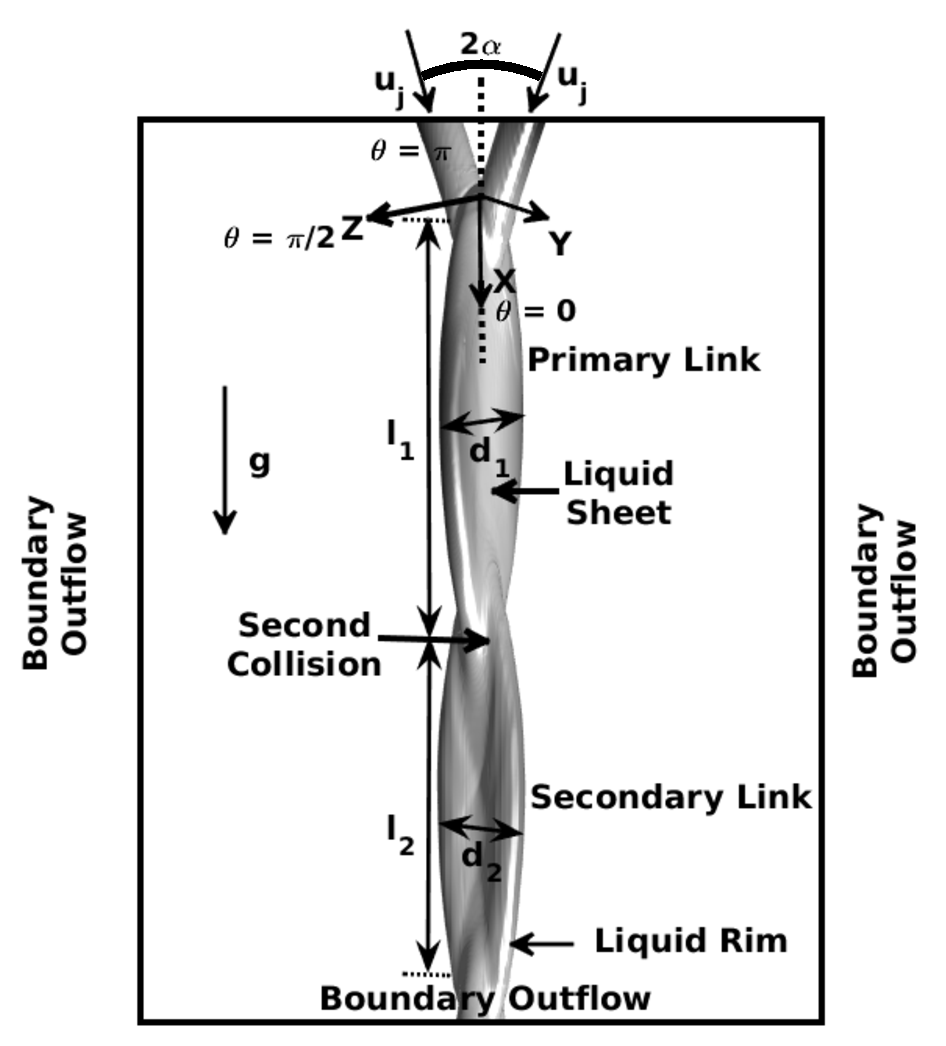
\includegraphics[width=0.5\linewidth]{schematic}
	\caption{}
	\label{Figure::schematic}
\end{figure}
\lipsum
\section{Numerical Formulation}\label{Appendix::Numerical}
%% Introduction to the problem
Collision of liquid jets has been studied using three-dimensional two-phase flow simulations using the finite volume framework for discretization and Volume Of Fluid (VOF) approach for interface tracking. Open source time-dependent, multi-fluid Navier-Stokes solver, Gerris is used for the current study \citep{Popinet2003}. Gerris has been successful used frequently by researchers, such as \cite{chen2013high,kumar2016physical,kumar2017bending}, to delve into similar problems in interfacial flows involving liquid sheets, jets and thin features like ligaments and films to capture intricate flow details and investigate the process. It invokes an adaptive mesh projection method for solution of incompressible continuity and momentum equations. The spatial discretization of the domain is undertaken using an octree based structured hierarchal grid system, which can be locally refined. Equation~\ref{Equation::mass} contains the mass conservation equation for the incompressible flow, which simply states that the velocity field ($V_i = V_1\hat{i} + V_2\hat{j} + V_3\hat{k}$) must be divergence free.   
\begin{equation} \label{Equation::mass}
\frac{\partial V_i}{\partial x_i} = 0
\end{equation}
The momentum equation for the incompressible Newtonian fluids solved for all three spatial coordinates can be summarized as given in equation~\ref{Equation::NS}. In the equation, the forces applied on the control volume chosen consist of the pressure in form of its gradient field ($\frac{\partial p}{\partial x_i}$), the volume specific body force due to gravitation ($\rho g_i$), the surface forces due to shear stress ($2\mu D_{ik}$, where $\mu)$ represents the coefficient of dynamic viscosity and $D_{ik}$ is the deformation tensor) and the interface specific surface tension force ($\sigma \kappa$, where $\sigma$ is the surface tension coefficient and $\kappa$ denotes the curvature of interface). 
\begin{equation} \label{Equation::NS}
\rho\left( \frac{\partial V_i}{\partial t} + V_k\frac{\partial V_i}{\partial x_k} \right) = -\frac{\partial p}{\partial x_i} + \frac{\partial (2\mu D_{ik})}{\partial x_k} + \sigma \kappa \delta_sm_i + \rho g_i
\end{equation}
Moreover, the surface tension term is multiplied with the Dirac distribution function ($\delta_s$) to ensure that the force by surface tension is concentrated at the interface having the normal vector $m_i$. Further, the deformation tensor $D_{ik}$ is defined using the symmetric part of the velocity field gradient as given in Equation~\ref{Equation::deformation}.
\begin{equation} \label{Equation::deformation}
D_{ik} = \frac{1}{2}\left(\frac{\partial V_i}{\partial x_k} + \frac{\partial V_k}{\partial x_i}\right)
\end{equation}
The Equation~\ref{Equation::NS} (Navier Stokes) implicitly implies the conservation of the mechanical energy. Moreover, the temperature variations are too small to affect the phenomenon being investigated and therefore, no thermal energy equation is employed. The interface tracking is undertaken using the Volume Of Fluid (VOF) approach. For this, a volume fraction (tracer) is defined as $\Psi(x_i,t)$, at the spatial and temporal instance of $x_i$ and $t$ respectively. Therefore, the density and viscosity for the study can be defined as given by Equation~\ref{Equation::general}. The Volume of Fluid approach implemented is a two-step process of interface reconstruction (based on the values of $\Psi$ and piecewise linear interface construction scheme, PLIC) along with geometric flux computation and interface advection. Equation~\ref{Equation::vof} represents the advection equation for the volume fraction field.
\begin{equation} \label{Equation::general}
A (\Psi) = \Psi A_1 + (1-\Psi)A_2 \: \: \:  \forall  \: A \in \{\rho, \mu\}
\end{equation}
\begin{equation} \label{Equation::vof}
\frac{\partial \Psi}{\partial t} + \frac{\partial(\Psi V_i)}{\partial x_i} = 0
\end{equation}
%% Time marching scheme
Second order accurate time discretization of momentum and continuity equations are carried out with time splitting algorithm as proposed by \cite{Chorin1968}, whereby an unconditionally stable corrector predictor time marching approach is adopted. A multi-grid solver is used for solution of the resulting pressure-Laplace equation. The advection term of the momentum equation $\left(V_k\frac{\partial V_i}{dx_k}\right)$ is estimated using the Bell-Colella-Glaz second-order unsplit upwind scheme \citep{bell1989second}, which requires the restriction to be set up on the time step between subsequent time steps based on the Courant-Friedrichs-Lewy (CFL) stability criteria as the estimation is stable only for CFL $<$ 1 \citep{popinet2009}. The details of the octree-based multi-level solver employed for the solution of the system of the equations can be found in the works of \cite{Popinet2003,popinet2009}. \\ 
%% Specific to this problem
Figure~\ref{Figure::schematic} illustrates the computational domain with dimensions 30$d_j$ x 10$d_j$ x 10$d_j$. The lateral surfaces are kept at a distance of $5d_j$ to avoid any biasing from the boundaries. These surfaces along with the bottom one are kept as standard boundary outflow. Two small liquid jets inclined at an angle of $\alpha$ from the vertical are initialized at the start of the simulation. The boundary condition on the top surface of the computational domain is that of liquid jet inlets, for which a parabolic velocity profile $\left(\left[2\left(1 - \left(\frac{2r}{d_j}\right)^2\right) \right]u_j\right)$ is patched, where $r$ is the radial location in the jet from its centerline, $d_j$ is the diameter of the liquid jets and $u_j$ is the average inlet velocity of the jet as illustrated in Figure~\ref{Figure::schematic}. We restrict ourselves in the laminar flow regime as the formation of stable liquid chains or sheet structures with closed rim is prominent in this regime. Following the Equations~\ref{Equation::mass} to~\ref{Equation::vof} and the boundary conditions, one can easily see that different features of these liquid sheets can be represented in terms of the kinematic and dynamic properties, such as jet velocity $\left(u_j\right)$, its diameter $\left(d_j\right)$, angle of impingement $\left(2\alpha\right)$, acceleration due to gravity $\left(g\right)$ and other physical properties, such as density of the fluid $\left(\rho\right)$, its viscosity $\left(\mu\right)$ and the coefficient of surface tension at the fluid-air interface. On dimensional analysis, different independent PI - terms are recognized as given in Equation~\ref{Equation::Pi}. On the left hand side we have different chain and link features, such as the length of individual lengths of the link, its maximum extent in the the plane of the formation of the liquid sheet, the average fluid velocity in the liquid sheet $\left(\frac{u_0}{u_j} = \frac{1}{u_j}\frac{\int_{0}^{2\pi}\frac{\int_{0}^{r_{max}}\frac{\int_{-h}^{h}\sqrt{u_iu_i}dy}{2h}dr}{r_{max}}d\theta}{2\pi} \right)$ and the thickness of the liquid sheet at different spatial locations $\left(\frac{h}{d_j}\right)$. Further, on the right hand side of the equation, different non-dimensional numbers can be recognized based on flow and geometric properties. The first term can be identified as the Froude number $\left(Fr = \frac{u_j}{\sqrt{gd_j}}\right)$, which acts as a measure of the relative strength of the inertia of the liquid jet and the force of gravity. Gravity is taken in the positive x-direction as shown in Figure~\ref{Figure::schematic}. Second term is the Bond number $\left(Bo = \frac{\rho gd_j^2}{\sigma}\right)$, used to account for the strength of the surface tension force as compared with the gravity body force on the chain structure. The viscosity comes into consideration with the term given by $\left(\frac{\mu}{\rho\sqrt{gd_j^3}}\right)$, which can be simplified as the ratio between the Reynolds number $\left(Re = \frac{\rho u_jd_j}{\mu}\right)$ and the Froude number of the jet ($Fr$).
\begin{equation}\label{Equation::Pi}
\left(\frac{l_i}{d_j},\frac{d_i}{d_j},\frac{u_0}{u_j},\frac{h}{d_j}\right) = \Pi\left(\frac{u_j}{\sqrt{gd_j}},\frac{\rho gd_j^2}{\sigma},\frac{\mu}{\rho\sqrt{gd_j^3}},\alpha\right)
\end{equation}
With the development of the above Mathematical model, it is necessary to check for mesh sensitivity to the solution and further validation with the experimental results present in the literature, which has been carried out in the next section.
\section{ Mesh Sensitivity Analysis and Model Validation}
\begin{figure*}
	\centering
	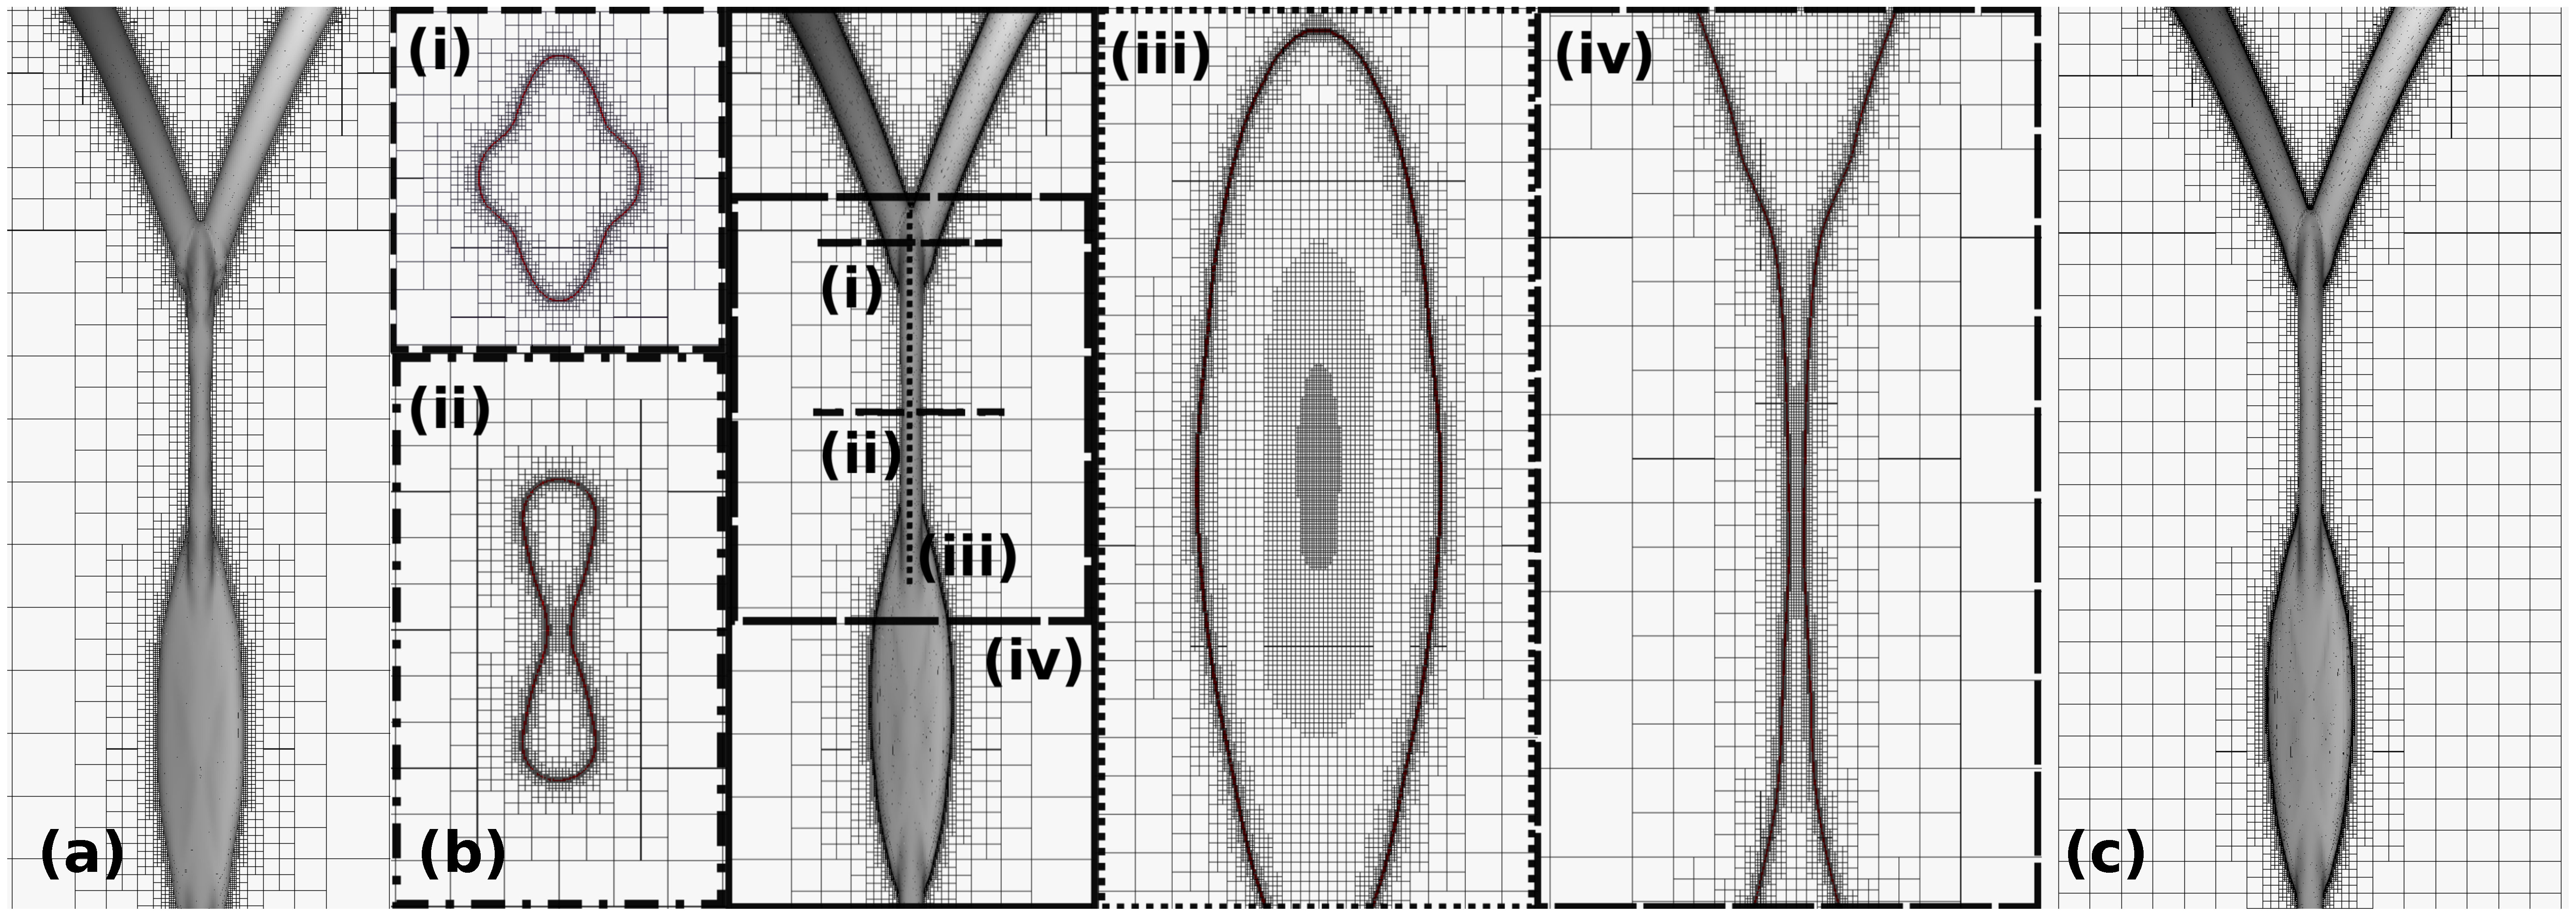
\includegraphics[width=\linewidth]{figGIS}
	\caption{}
	\label{Figure::GISfigures}
\end{figure*}
Sensitivity to the mesh refinement is analyzed in this section along with validation of the numerical results. Gerris uses an adaptive octree mode of refinement as illustrated in Figure~\ref{Figure::GISfigures}. It is necessary to capture the smallest features of the flow, in this case, the thickness of the liquid sheet. The multi-level grid structure adapts itself according to the gradient of the tracer $\Psi$, which implies that the structured octree mesh is finest at the interface between the two fluids. \cite{hasson1964thickness} gave a simple expression to quantify the thickness of the liquid sheet which takes the form of Equation~\ref{Equation::hrHassaon}.
\begin{equation}\label{Equation::hrHassaon}
\frac{hr}{d_j^2} = 	\frac{1}{4}\frac{sin^3\alpha}{(1-cos\theta\:cos\alpha)^2}
\end{equation}
Although the minimum of Equation~\ref{Equation::hrHassaon} occurs at $\theta \to \pi$, it must be noted that the decrement in thickness is more because of the increase in radial distance downstream of the first collision point $\left(h \propto \frac{1}{r}\right)$, which is maximum near low azimuthal angles (Figure~\ref{Figure::GISfigures}(b - iv)), just upstream of the second collision point. This happens because the fluid velocity increases as the gravitational potential is converted to kinetic energy and the thickness decreases to keep the mass flow rate constant. An order of magnitude analysis reveals that $\frac{hr}{d_j^2} \sim 1$ for the minimum thickness at $2\alpha = \frac{\pi}{2}$ in the range of our numerical simulations. Therefore, $\frac{d_j}{\delta l} \sim 10\frac{r_{max}}{d_j}$ can be used as an imperative starting point for the grid independence study. The factor of 10 is included to have at least 10 grid points across the smallest length scale for the structure to be fully resolved \citep{ling2015multiscale}, else the sheet thickness will be equal to the minimum grid size and the sheet would break at the cost of being unresolved \citep{chen2013high}.
\begin{figure}
	\centering
	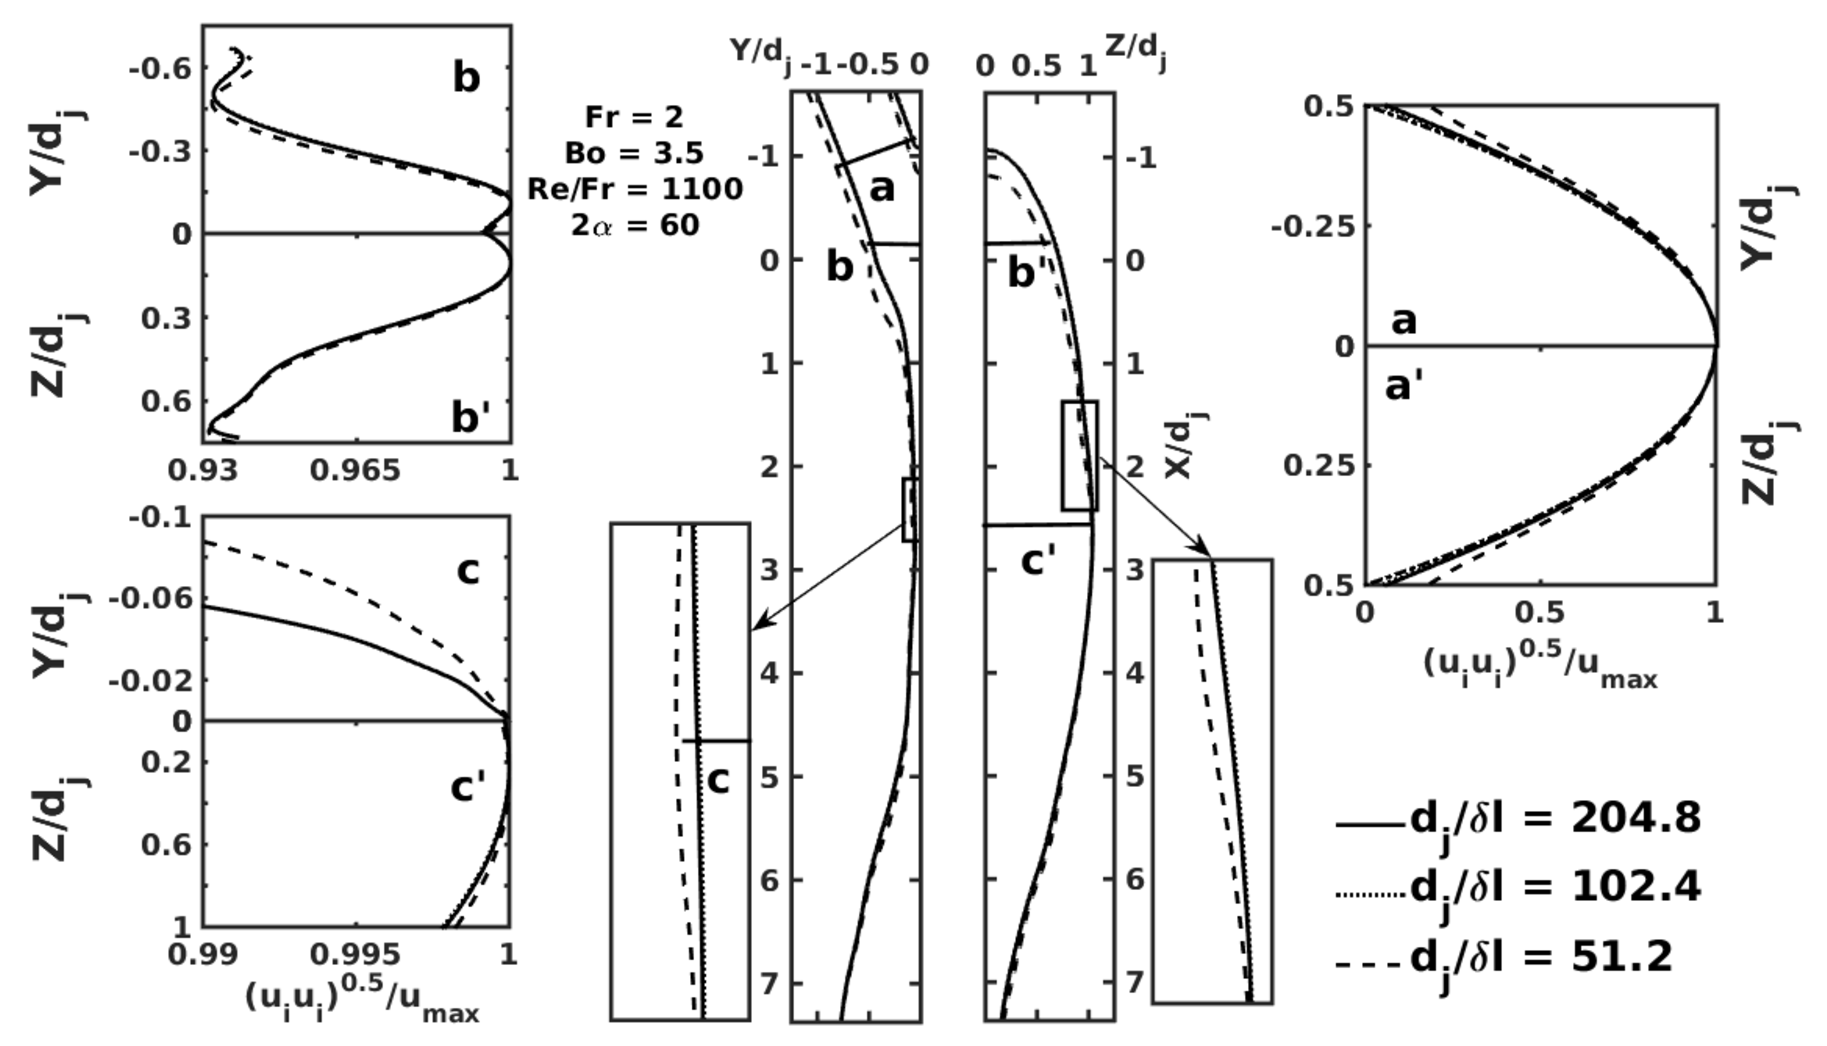
\includegraphics[width=\linewidth]{gis}
	\caption{}
	\label{Figure::GISplots}
\end{figure}
Figure~\ref{Figure::GISplots} gives a representative case employed for the grid independence study. Applying above discussed arguments, $\frac{d_j}{\delta l} \sim 70$ (Figure~\ref{Figure::GISfigures}(a)) should be ideal for the simulations. It can be  clearly seen that the variations in the results such as the contour of the tracer (volume fraction) and velocity profiles at different locations downstream of the collision point, saturate if the refinement is increased from $\frac{d_j}{\delta l} = 102.4$ (Figure~\ref{Figure::GISfigures}(b)) to $204.8$ (Figure~\ref{Figure::GISfigures}(c)). Moreover, the later requires more computational power and time. Therefore, a refinement level of $\frac{d_j}{\delta l} = 102.4$ is employed for this case. A similar analysis is carried out for all the cases reported in the present study initiated with $\frac{d_j}{\delta l} = 10\frac{r_{max}}{d_j}$, with $r_{max} = 10d_j$. If the sheet is still not fully resolved or the maximum radial extent goes higher that $10d_j$, the refinement level is increased.\\
\begin{table}[]
	\caption{Performance data of the processors used for simulations to determine the refinement level in the Grid Independence Study. The simulations are done using four Intel Core i7-6500U CPU having clock speed of 2.5GHz each and 8 GB RAM.}
	\label{Table::cpu}
	\centering
	\begin{tabular}{@{}cc@{}}
		\hline
		\begin{tabular}[c]{@{}c@{}} $\: \: \: \: \: \: \: \: \: \left(\frac{d_j}{\delta l}\right)_{max}$ \end{tabular} & \begin{tabular}[c]{@{}c@{}} $\: \: \: \: \: \: \: \: \: \left(\frac{t_{CPU}}{t_{actual}}\right)$ \\ $\: \: \: \: \: \: \: \: \:$(days/s) \end{tabular}\\ \hline
		51.2 & $\sim 20$\\
		102.4 & $\sim 28$ \\	
		204.8 & $\sim 60$ \\	\hline
	\end{tabular}
\end{table}
\begin{figure}
	\centering
	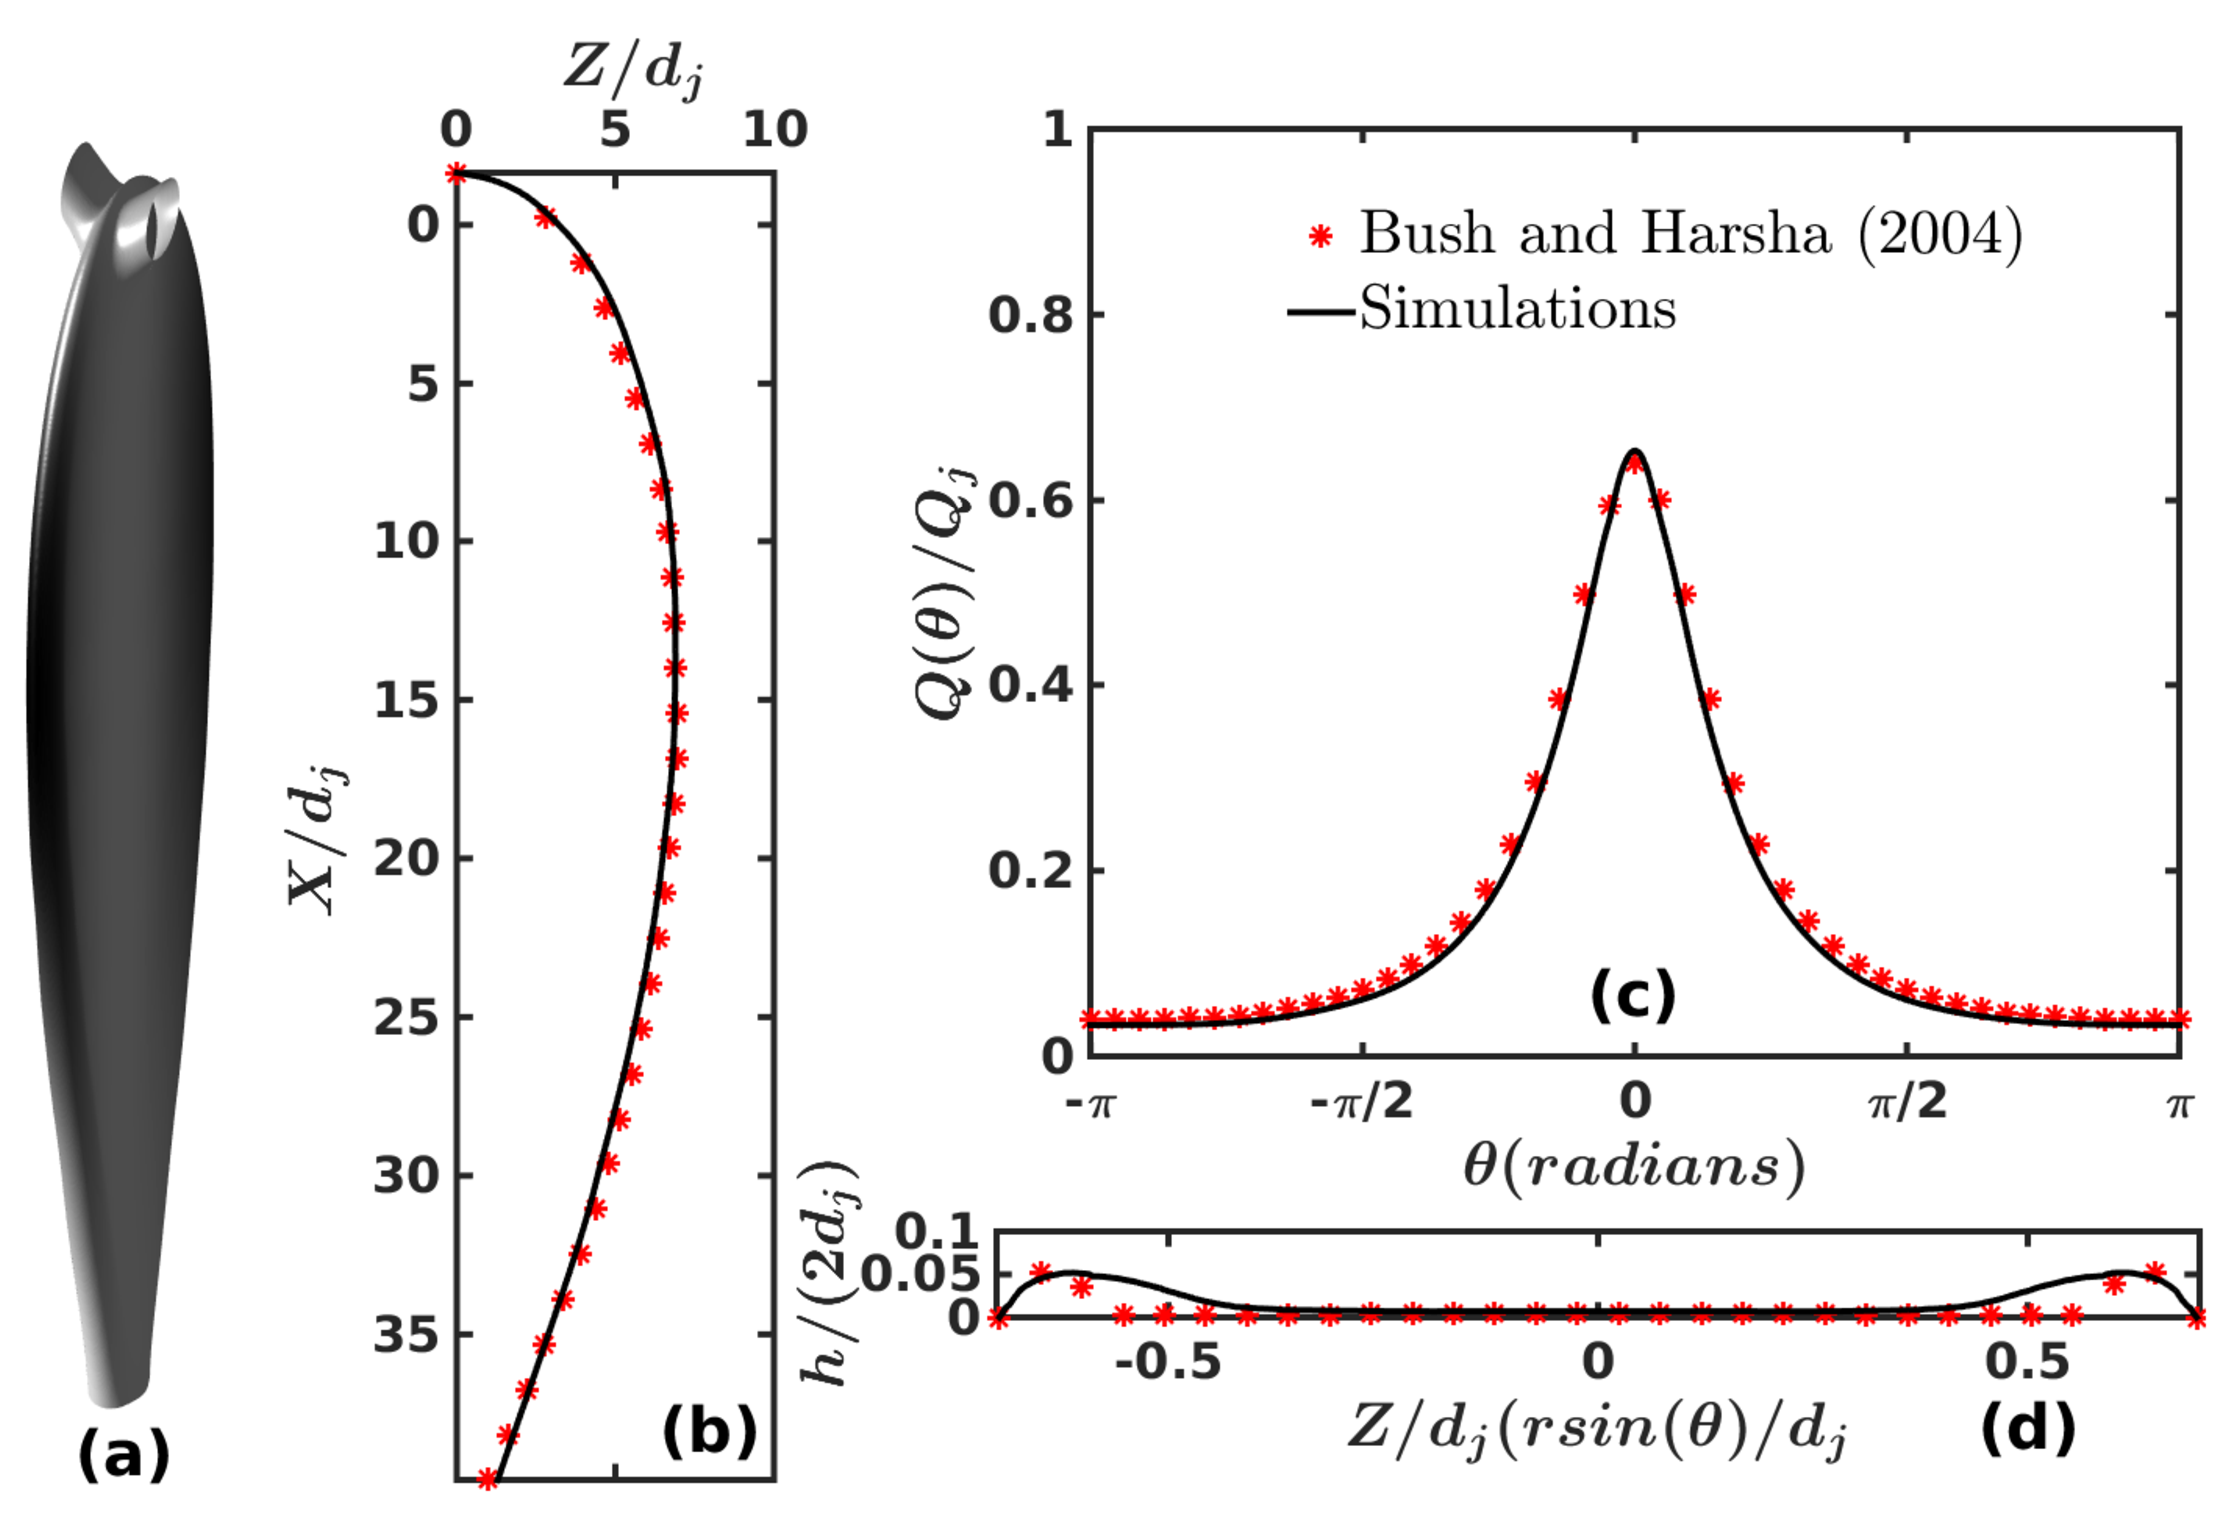
\includegraphics[width=\linewidth]{validation}
	\caption{}
	\label{Figure::validation}
\end{figure}
%%%%%%%
******************************************************\\
Next, we use the experimental results obtained by \cite{bush2004collision} to validate the employed numerical model. Figure~\ref{Figure::validation} presents a description of the results of this test. The first link of the chain structure formed is illustrated in Figure~\ref{Figure::validation}(a), with matching between the experimentally obtained boundary of the link and the contour generated from numerical simulations shown in Figure~\ref{Figure::validation}(b). In order to ensure that all\\
********************************************************
%%%%%%%%%%   
\lipsum[1]
\section{Formation of the chain}
\lipsum[1]
\subsection{Towards the steady state}

\begin{figure}[H]
	\centering
	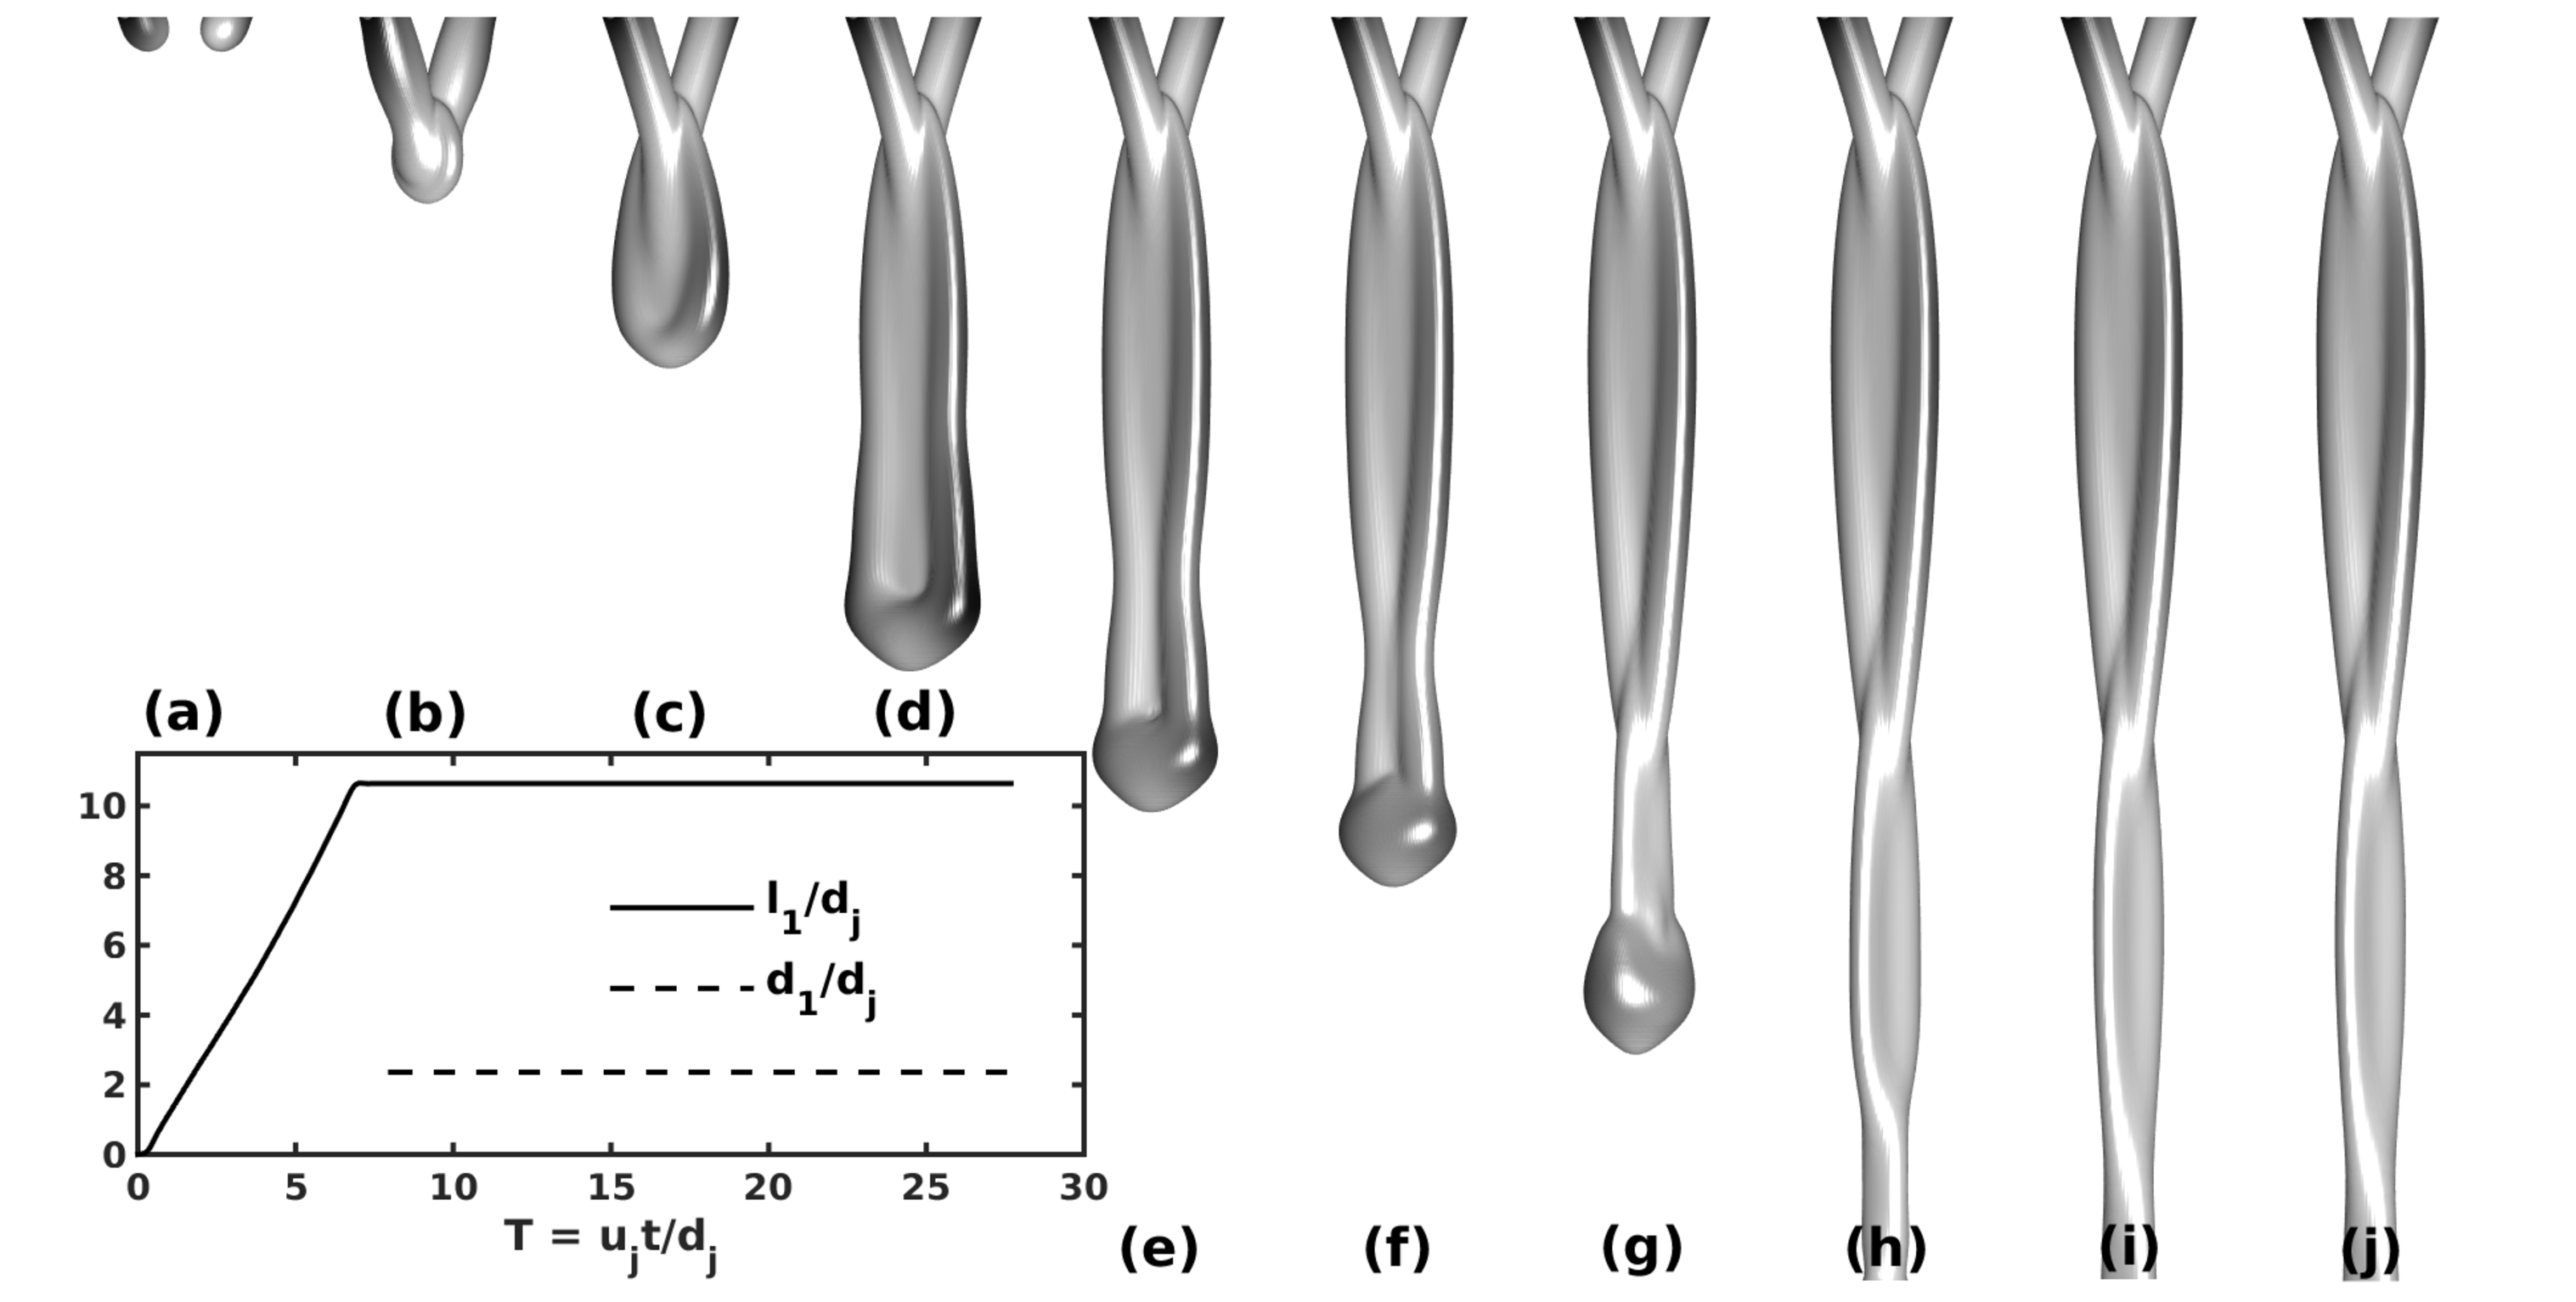
\includegraphics[width=\linewidth]{fig0}
	\caption{Transition to the steady state fluid-links chain formed by collision of laminar jets. The figure illustrates the transient period through the temporal advancement from (a) pre-collision symmetric jets to $T (\frac{u_jt}{d_j}) = $ (b) 1.5, (c) 4, (d) 5, (e) 5.5, (f) 6.5, (g) 8.5, (h) 16.5, (i) and (j) 20}
	\label{Figure::transient}
\end{figure}
\lipsum[1]
\subsection{Phase contours for different cases}
\lipsum[1]
\begin{figure*}
	\centering
	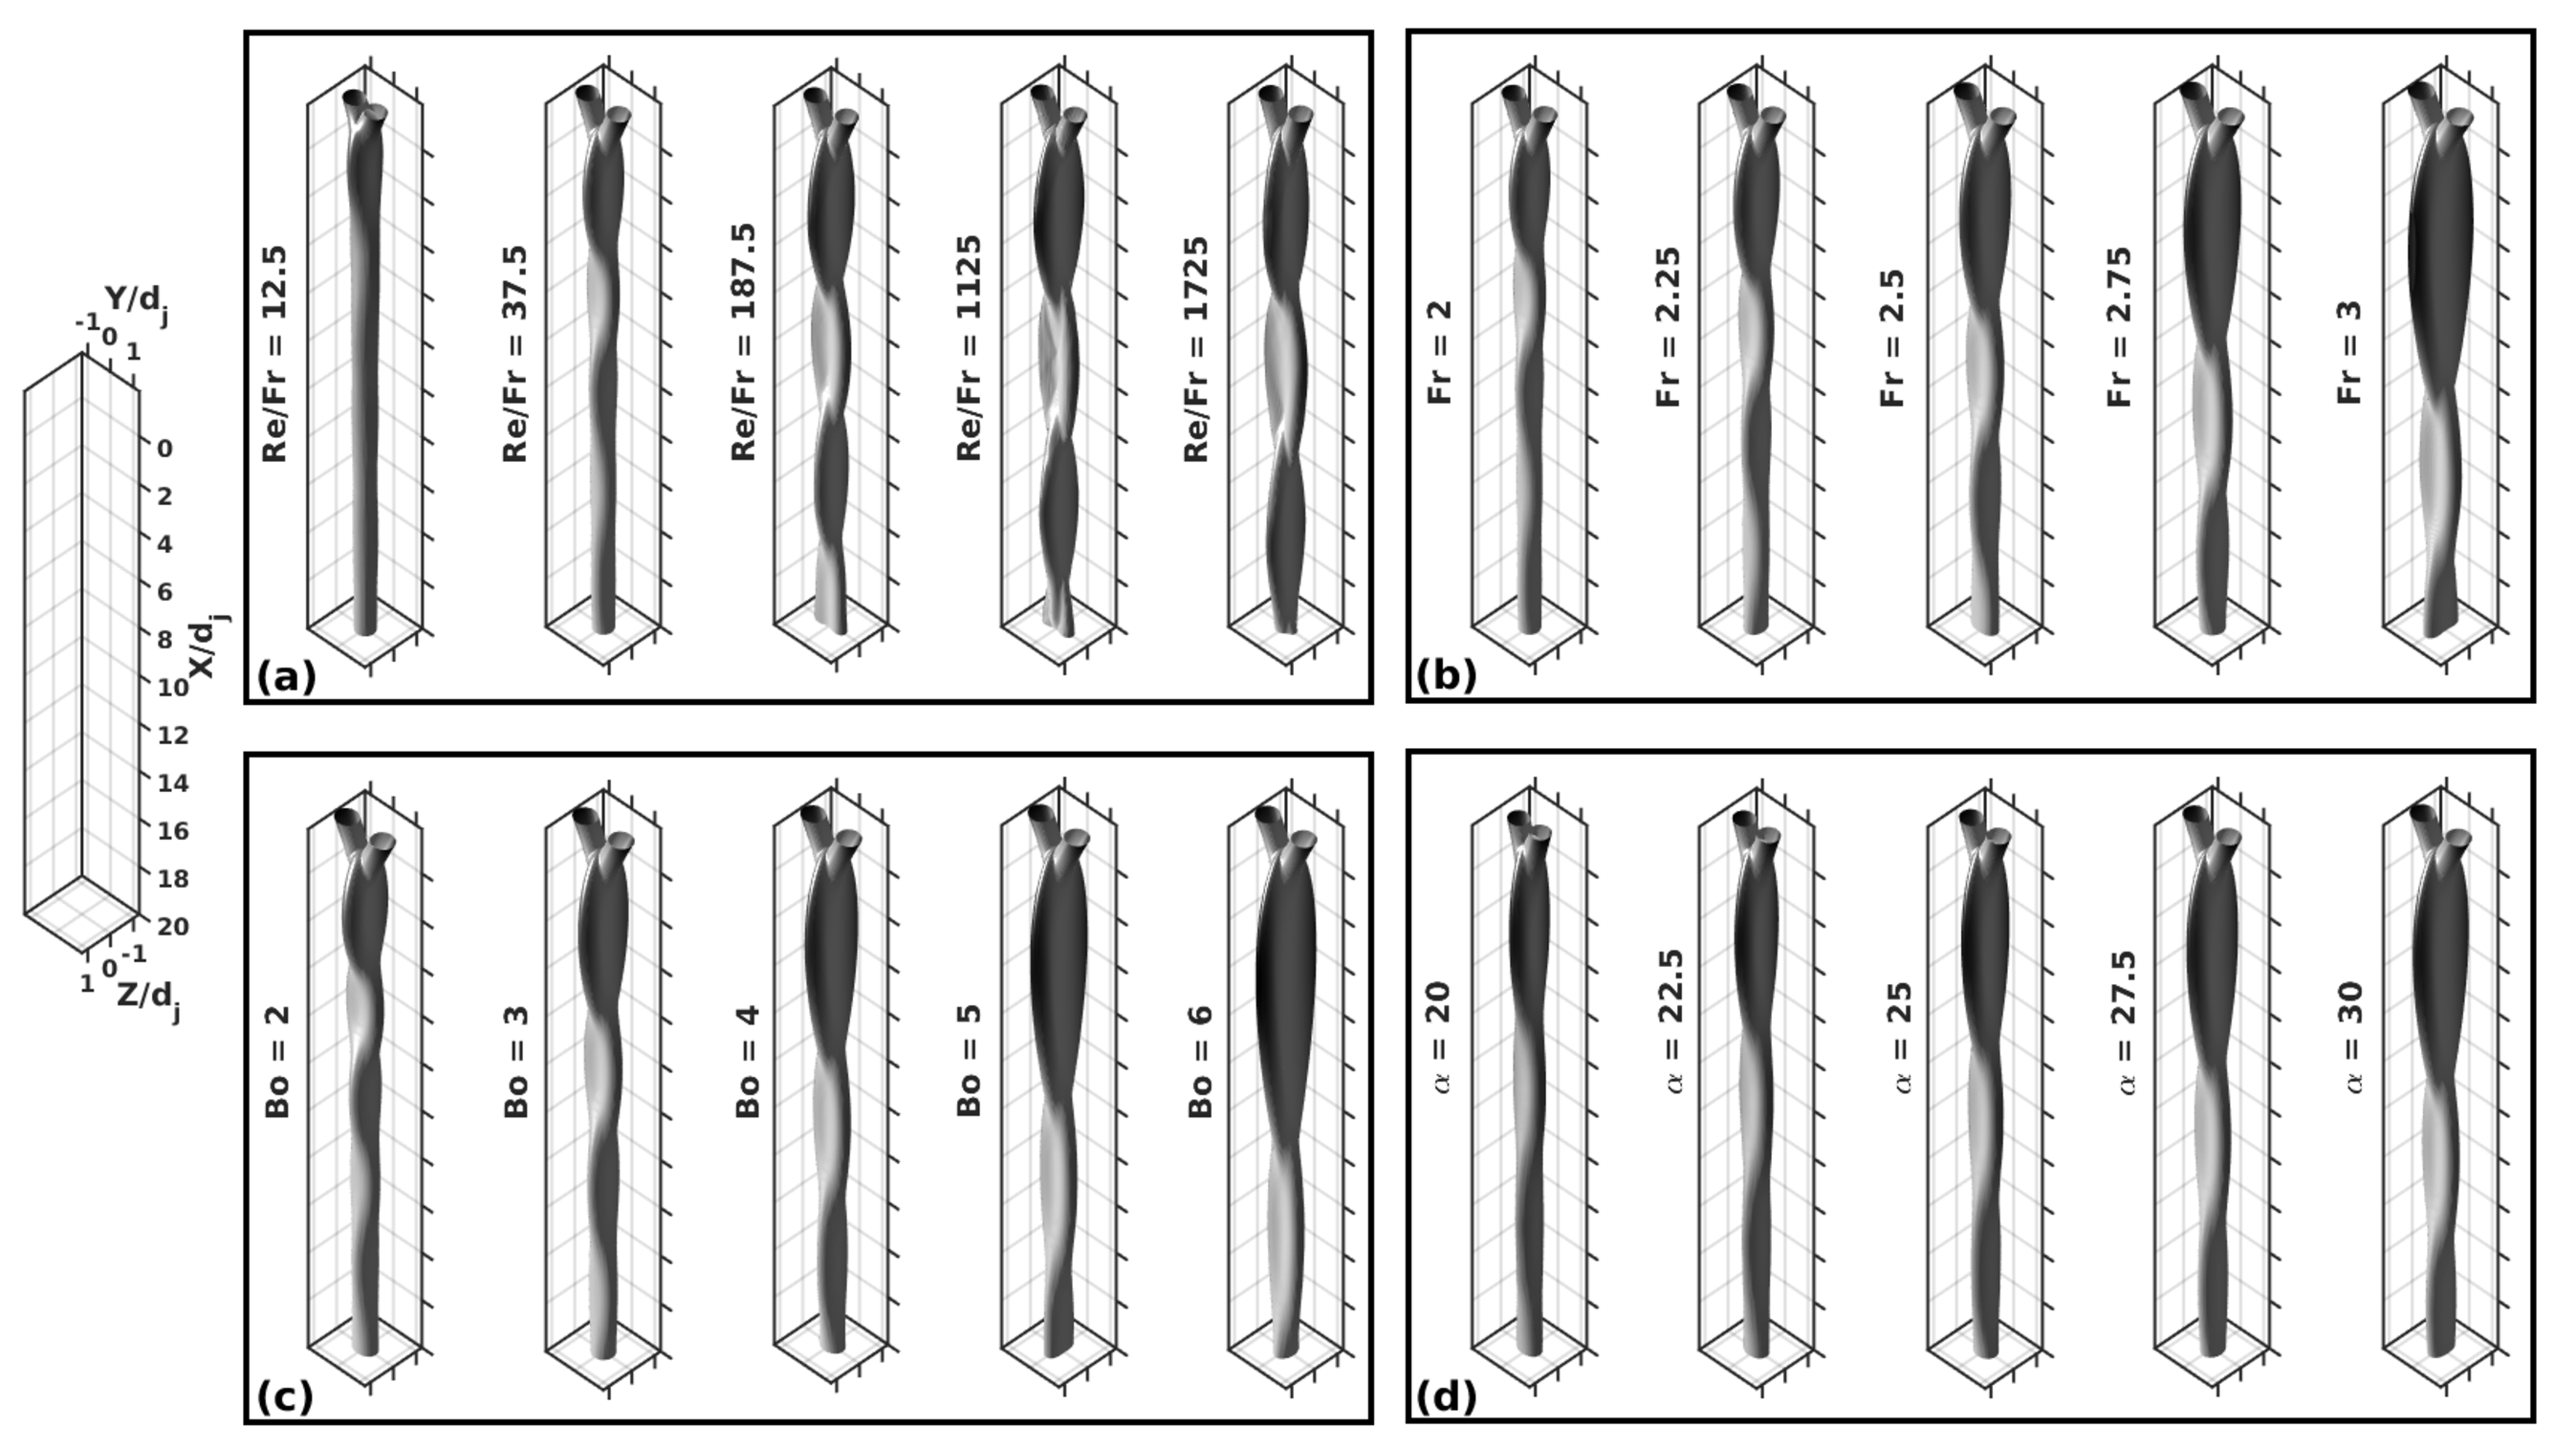
\includegraphics[width=\linewidth]{phaseContours}
	\caption{}
	\label{Figure::phaseContours}
\end{figure*}
\begin{figure}
	\centering
	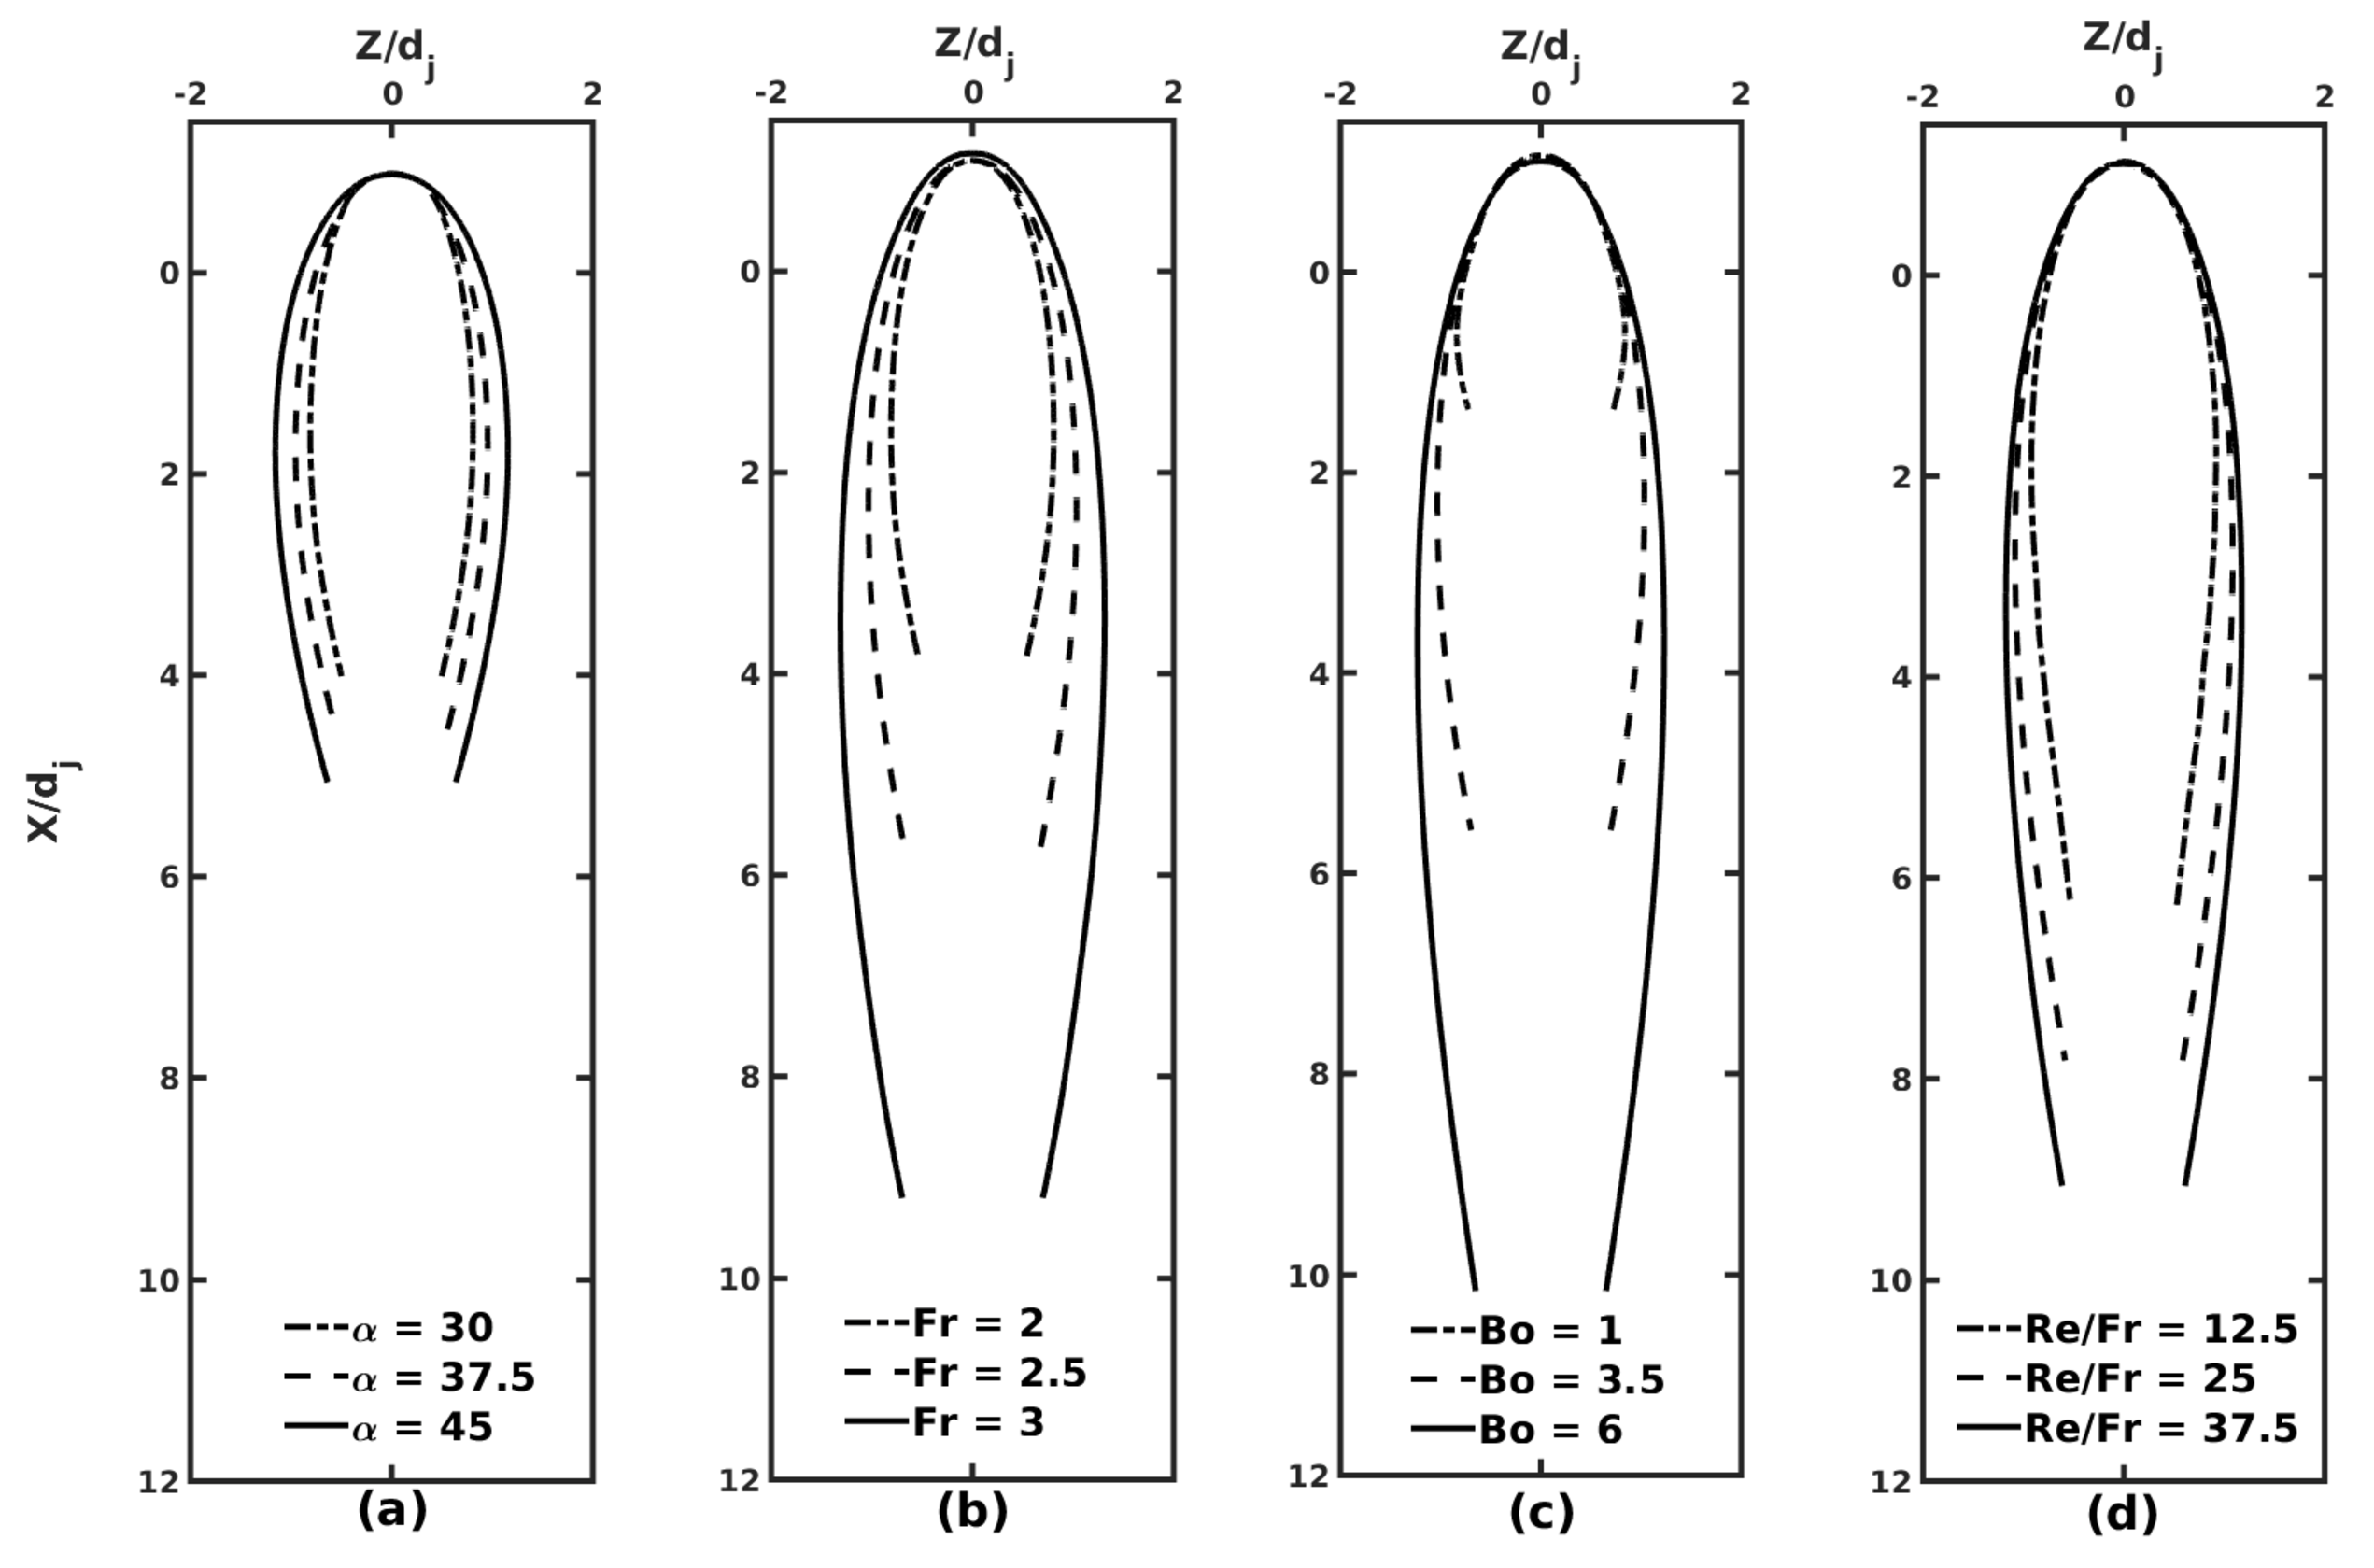
\includegraphics[width=\linewidth]{finalContour}
	\caption{}
	\label{Figure::finalContours}
\end{figure}
\lipsum
\section{Predicting the shape of the first link}
\lipsum[1]
\subsection{Co-relation model}
\lipsum[1]
\begin{figure}[H]
	\centering
	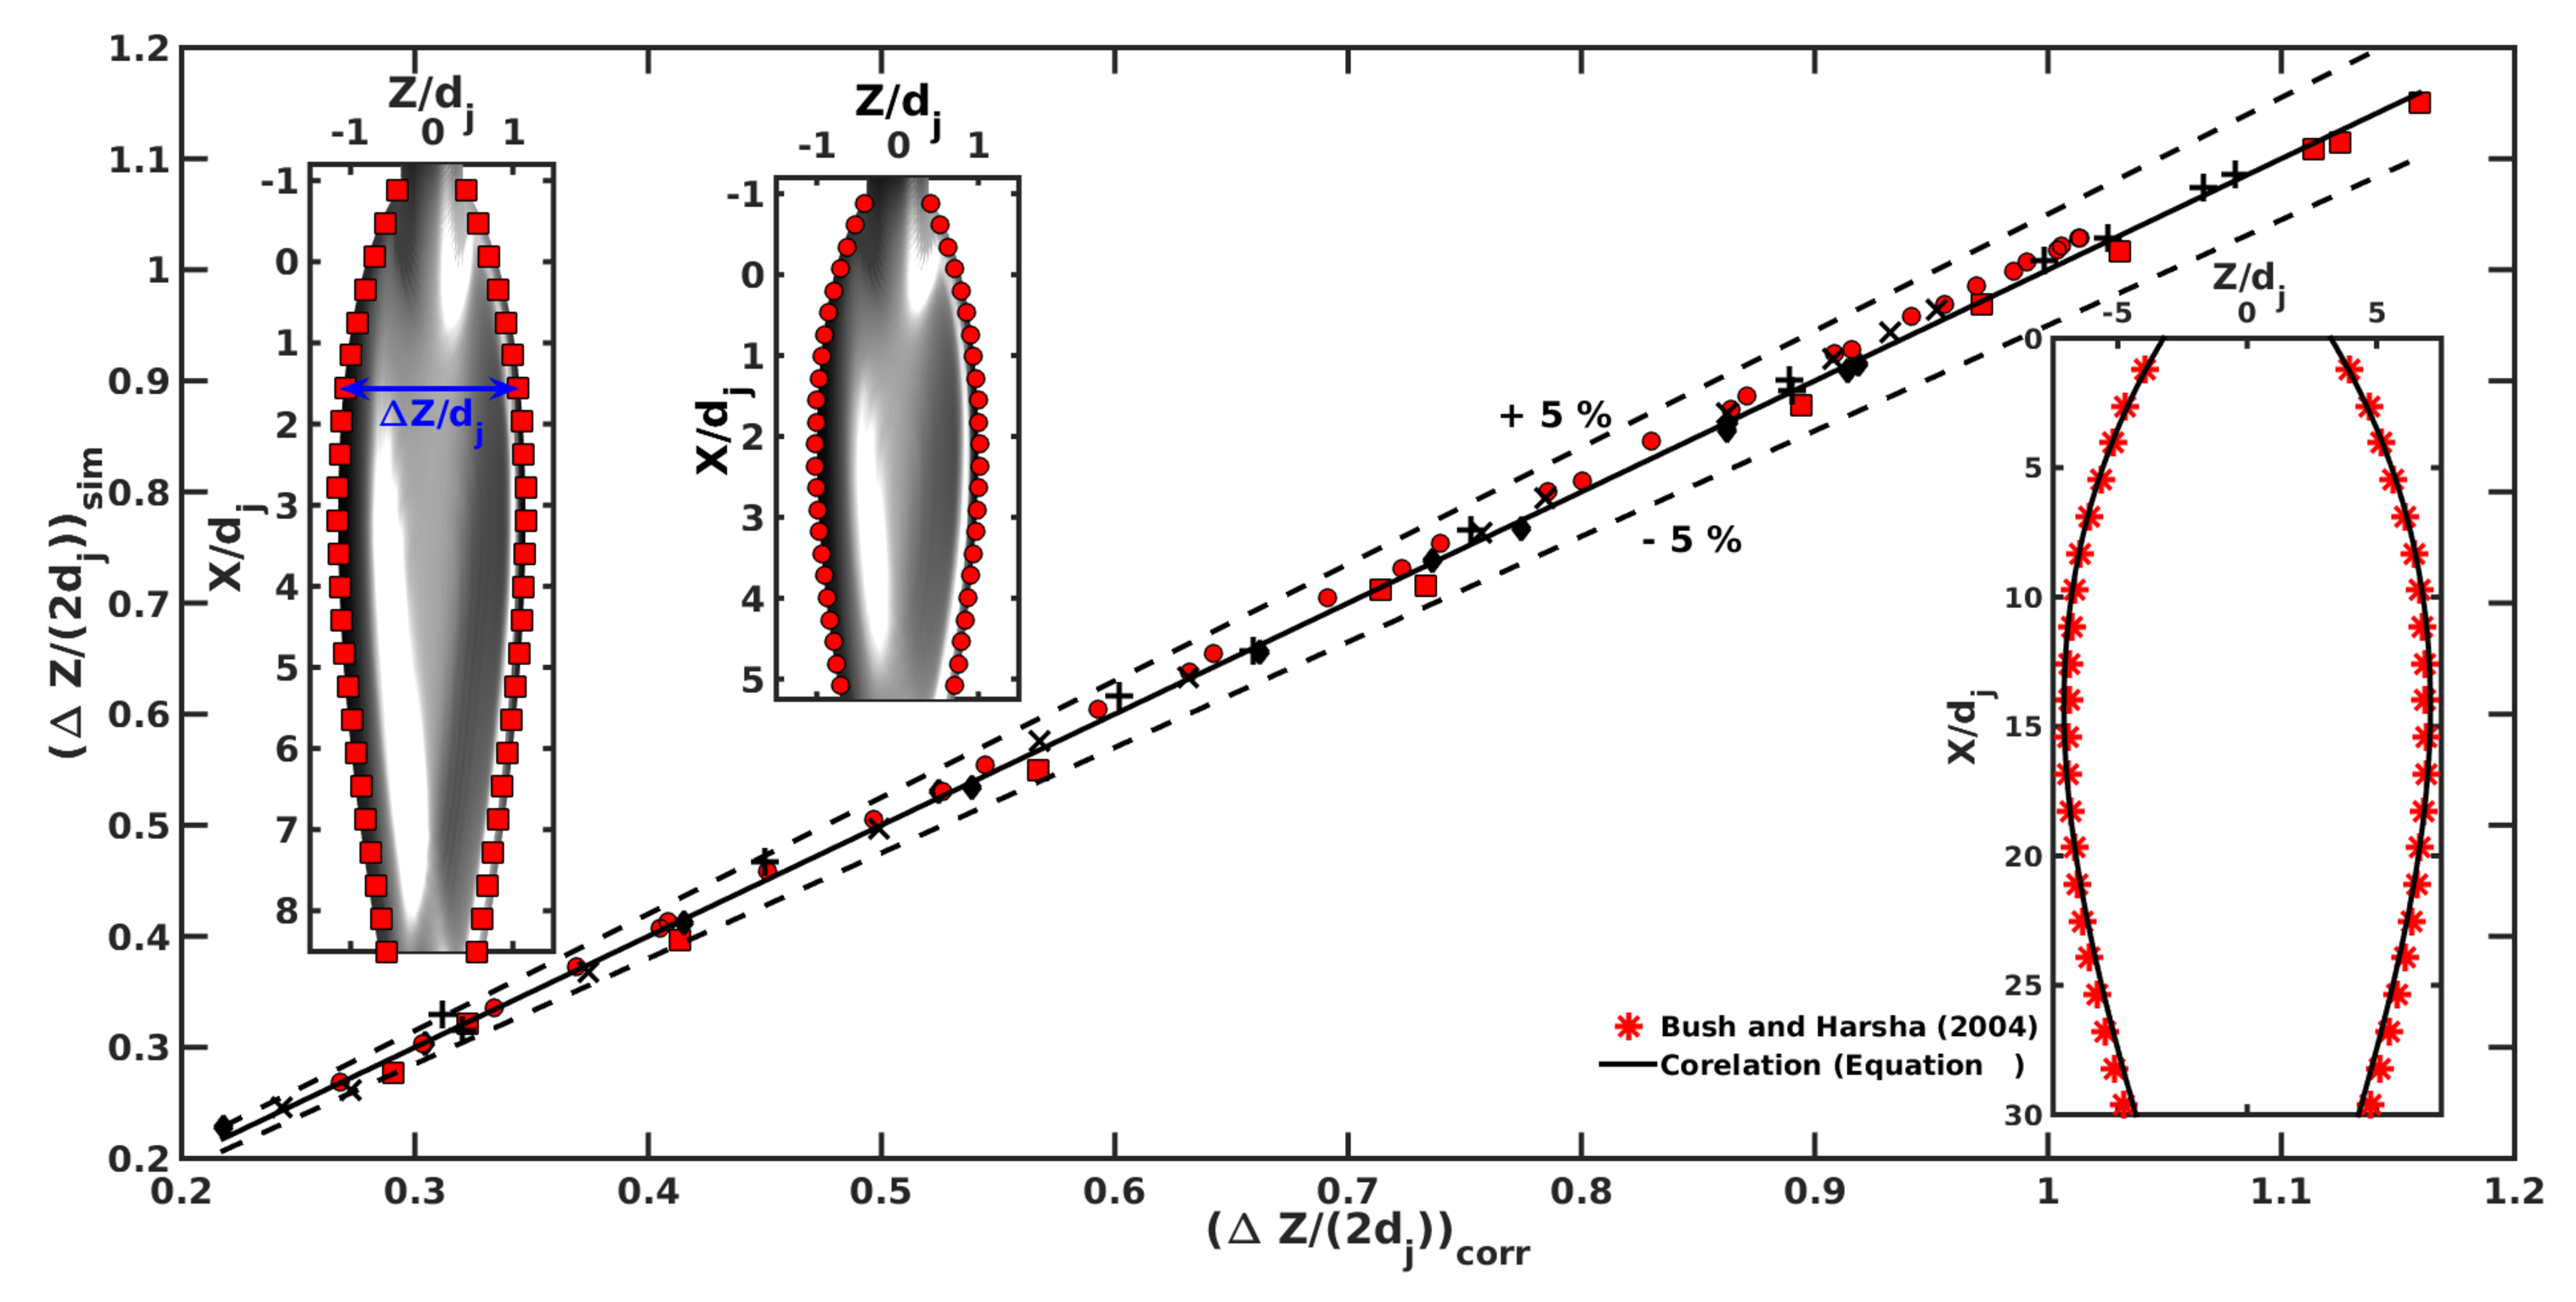
\includegraphics[width=\linewidth]{corelatehx}
	\caption{$\alpha$ = 30, $Fr$ = 2.5, $Bo$ = 5 and $Re/Fr$ = 34 (\protect\MarkerSquareRed); $\alpha$ = 30, $Fr$ = 2.5, $Bo$ = 4 and $Re/Fr$ = 34 (+); $\alpha$ = 30, $Fr$ = 2.5, $Bo$ = 2.3 and $Re/Fr$ = 20 (\protect \MarkerDiamondBlack); $\alpha$ = 25, $Fr$ = 2.5, $Bo$ = 4.57 and $Re/Fr$ = 34 ($\times$) and $\alpha$ = 30, $Fr$ = 2.5, $Bo$ = 3.75 and $Re/Fr$ = 20 (\protect \MarkerCircleRed) }
	\label{Figure::corelatehx}
\end{figure}
\lipsum[1]
\subsection{Analytical model}
\lipsum[1]
\begin{figure}
	\centering
	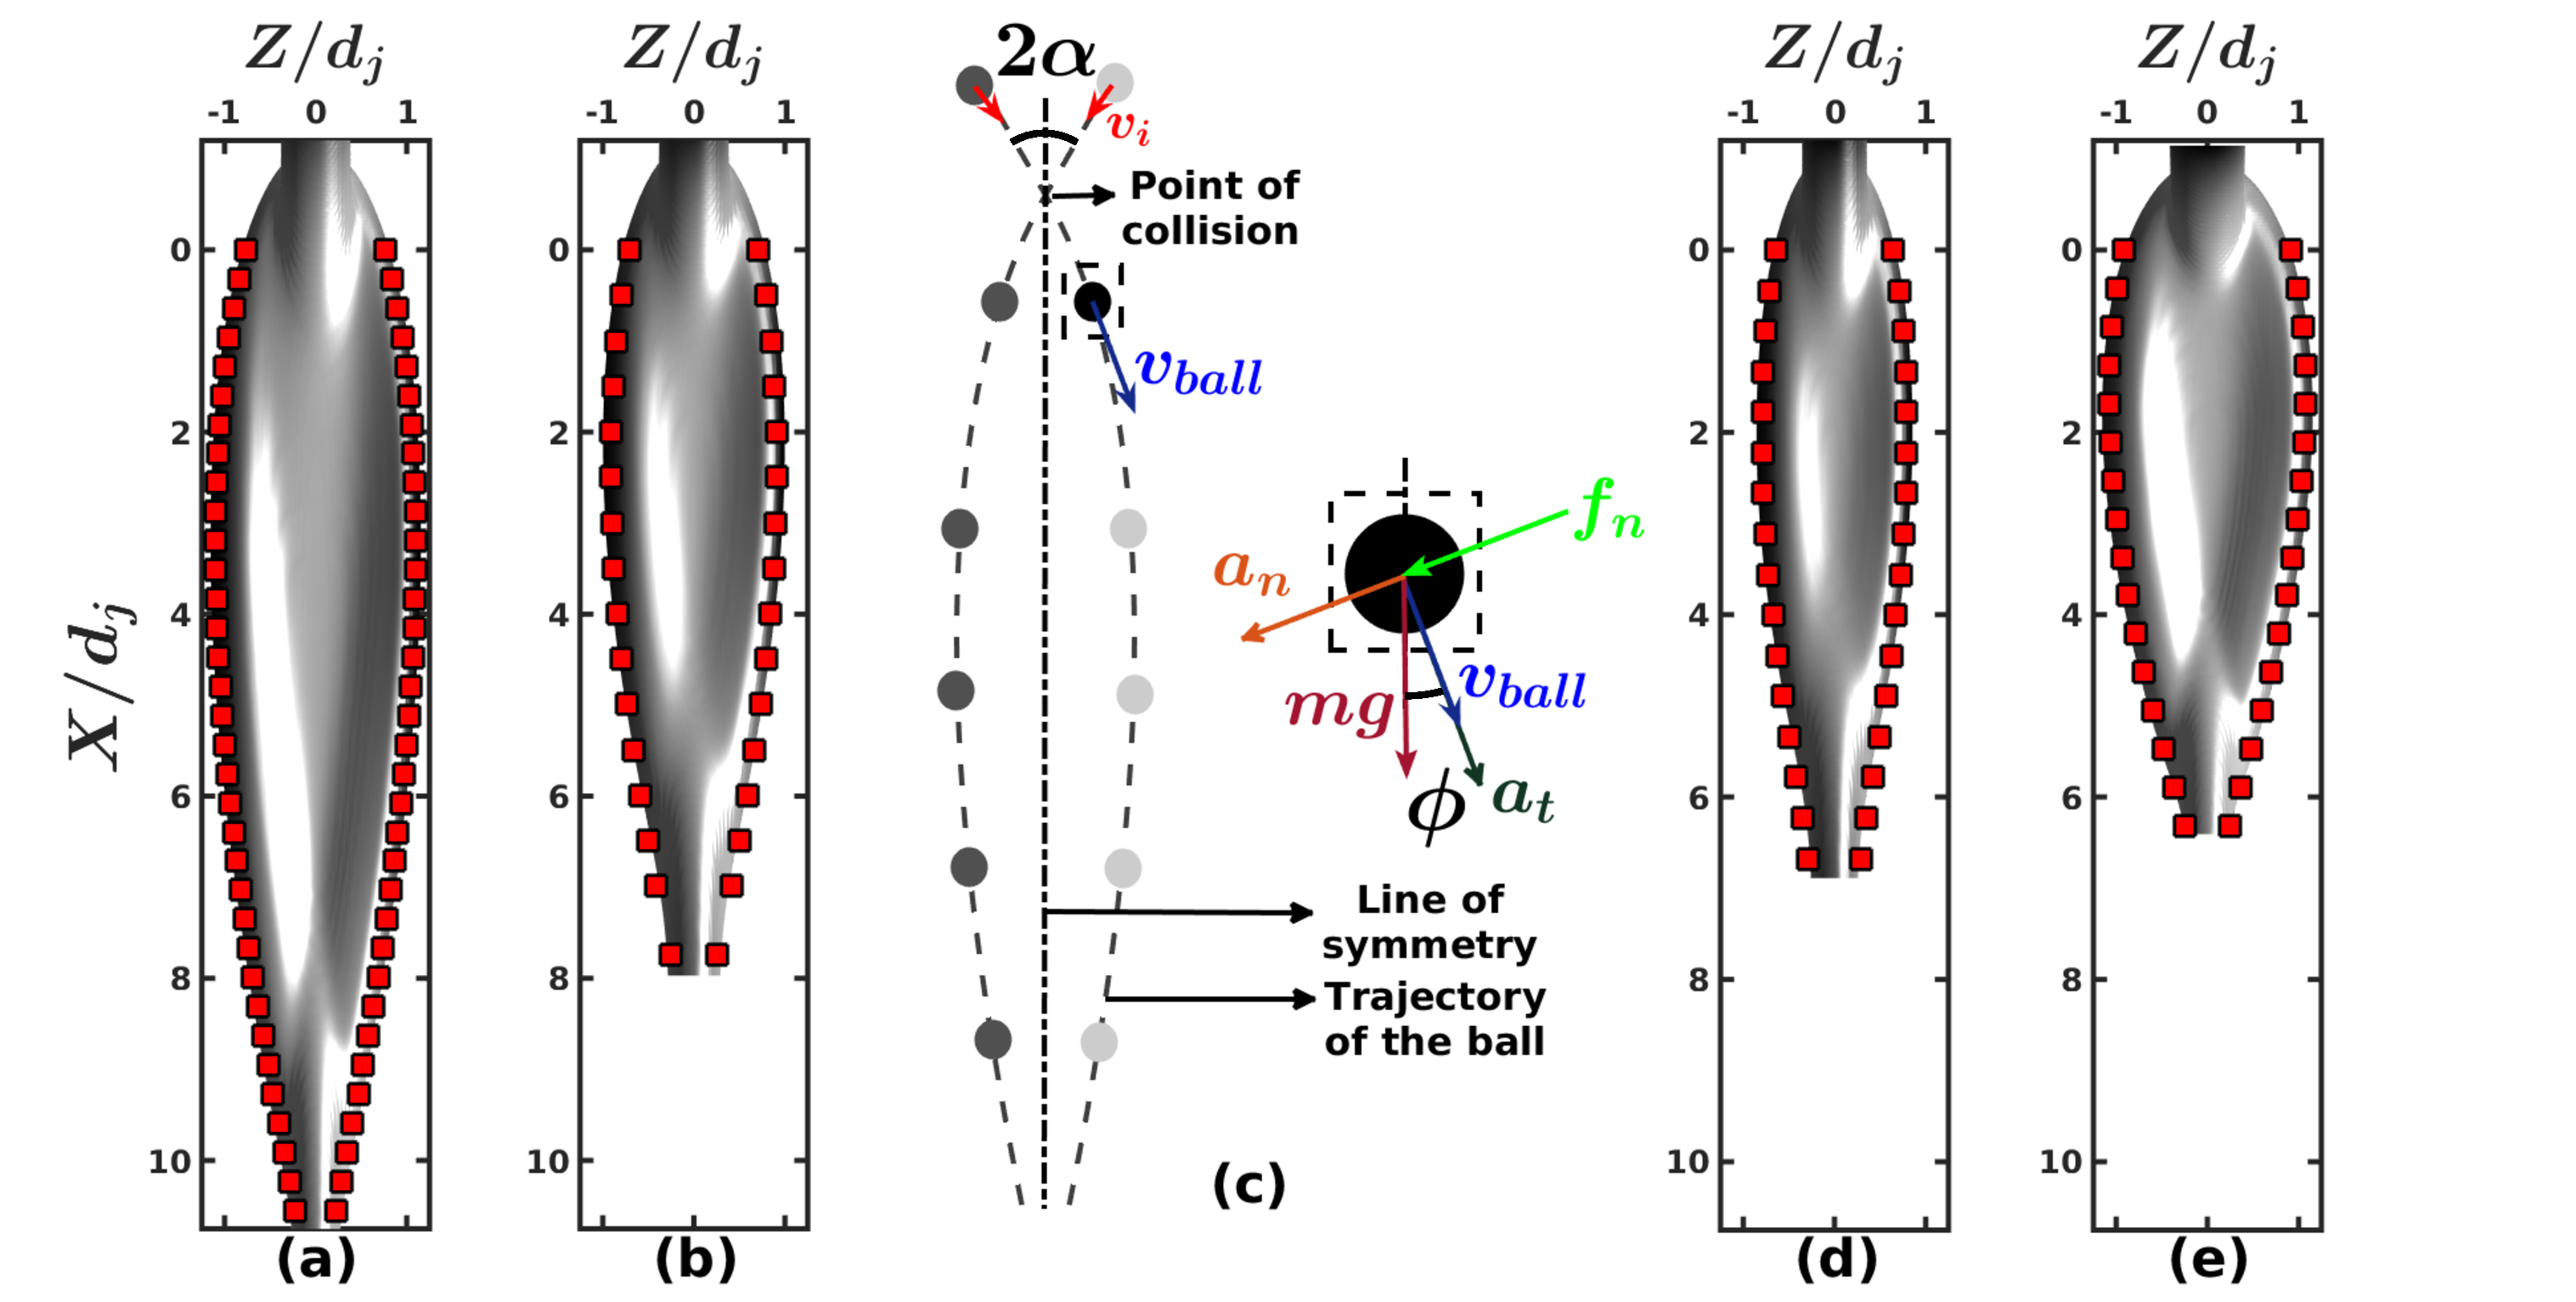
\includegraphics[width=\linewidth]{analytical}
	\caption{}
	\label{Figure::analytical}
\end{figure}
\lipsum[1]
\section{Velocity Field Description}
\lipsum[1]
\section{Second - Collision}
\begin{figure}[H]
	\centering
	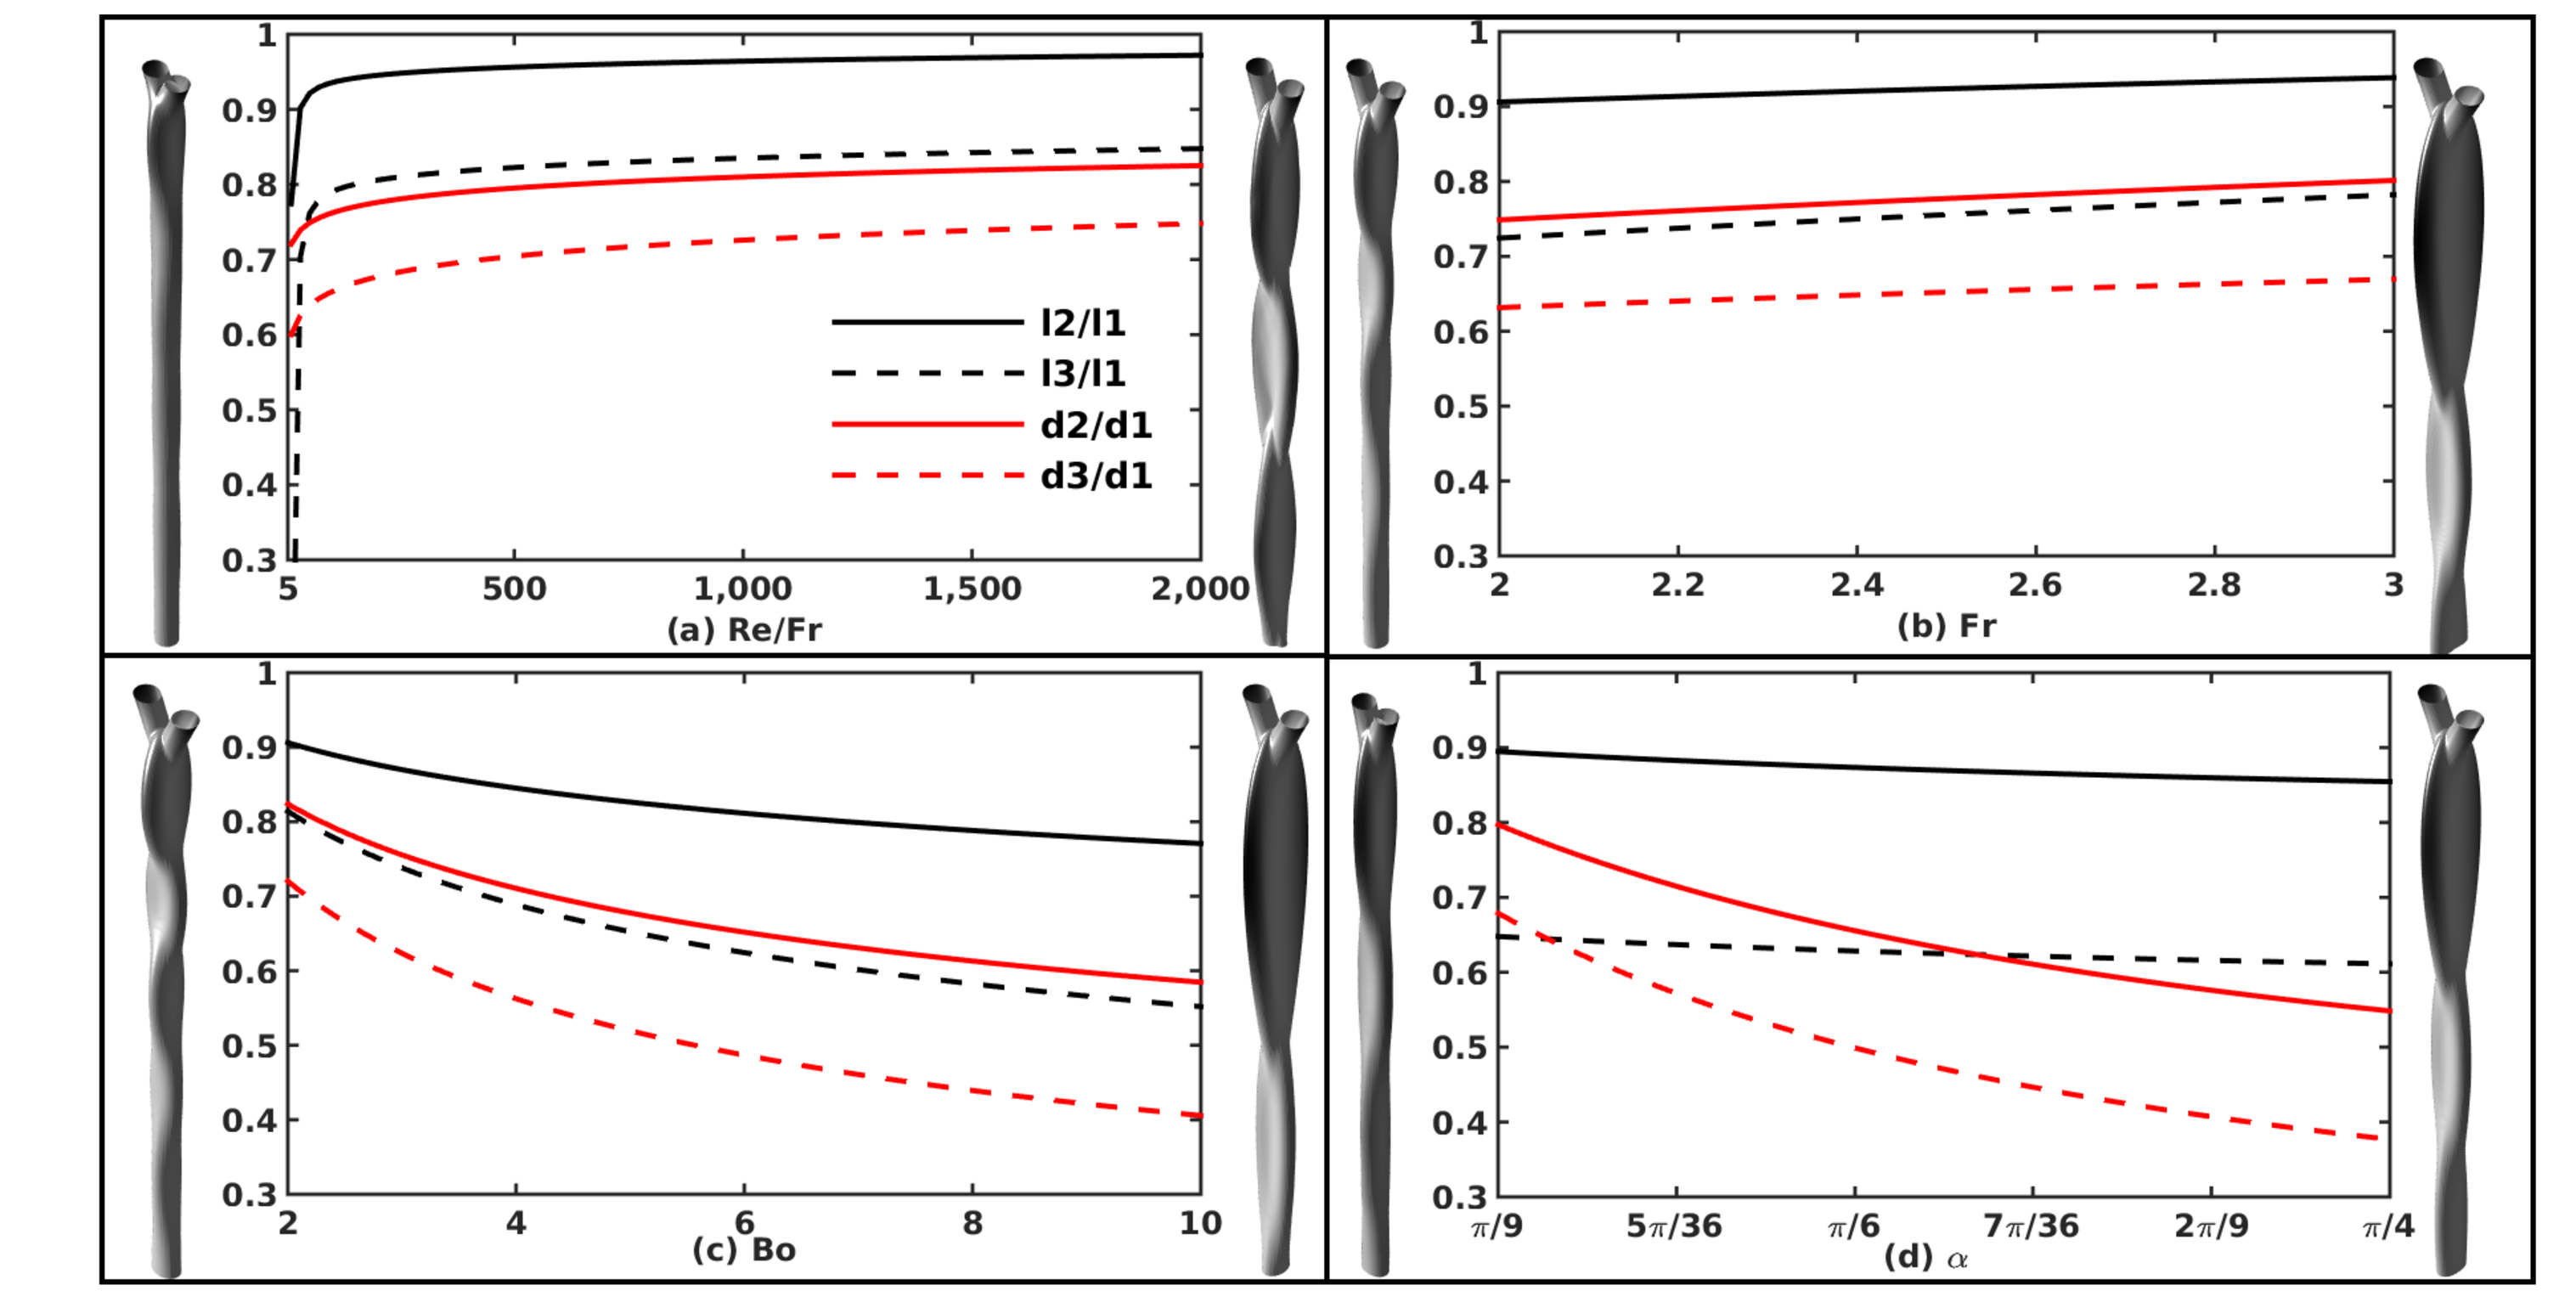
\includegraphics[width=\linewidth]{lil1did1}
	\caption{}
	\label{Figure::lil1}
\end{figure}
\lipsum[1]
\subsection{Twisting of streamlines}
\begin{figure}[H]
	\centering
	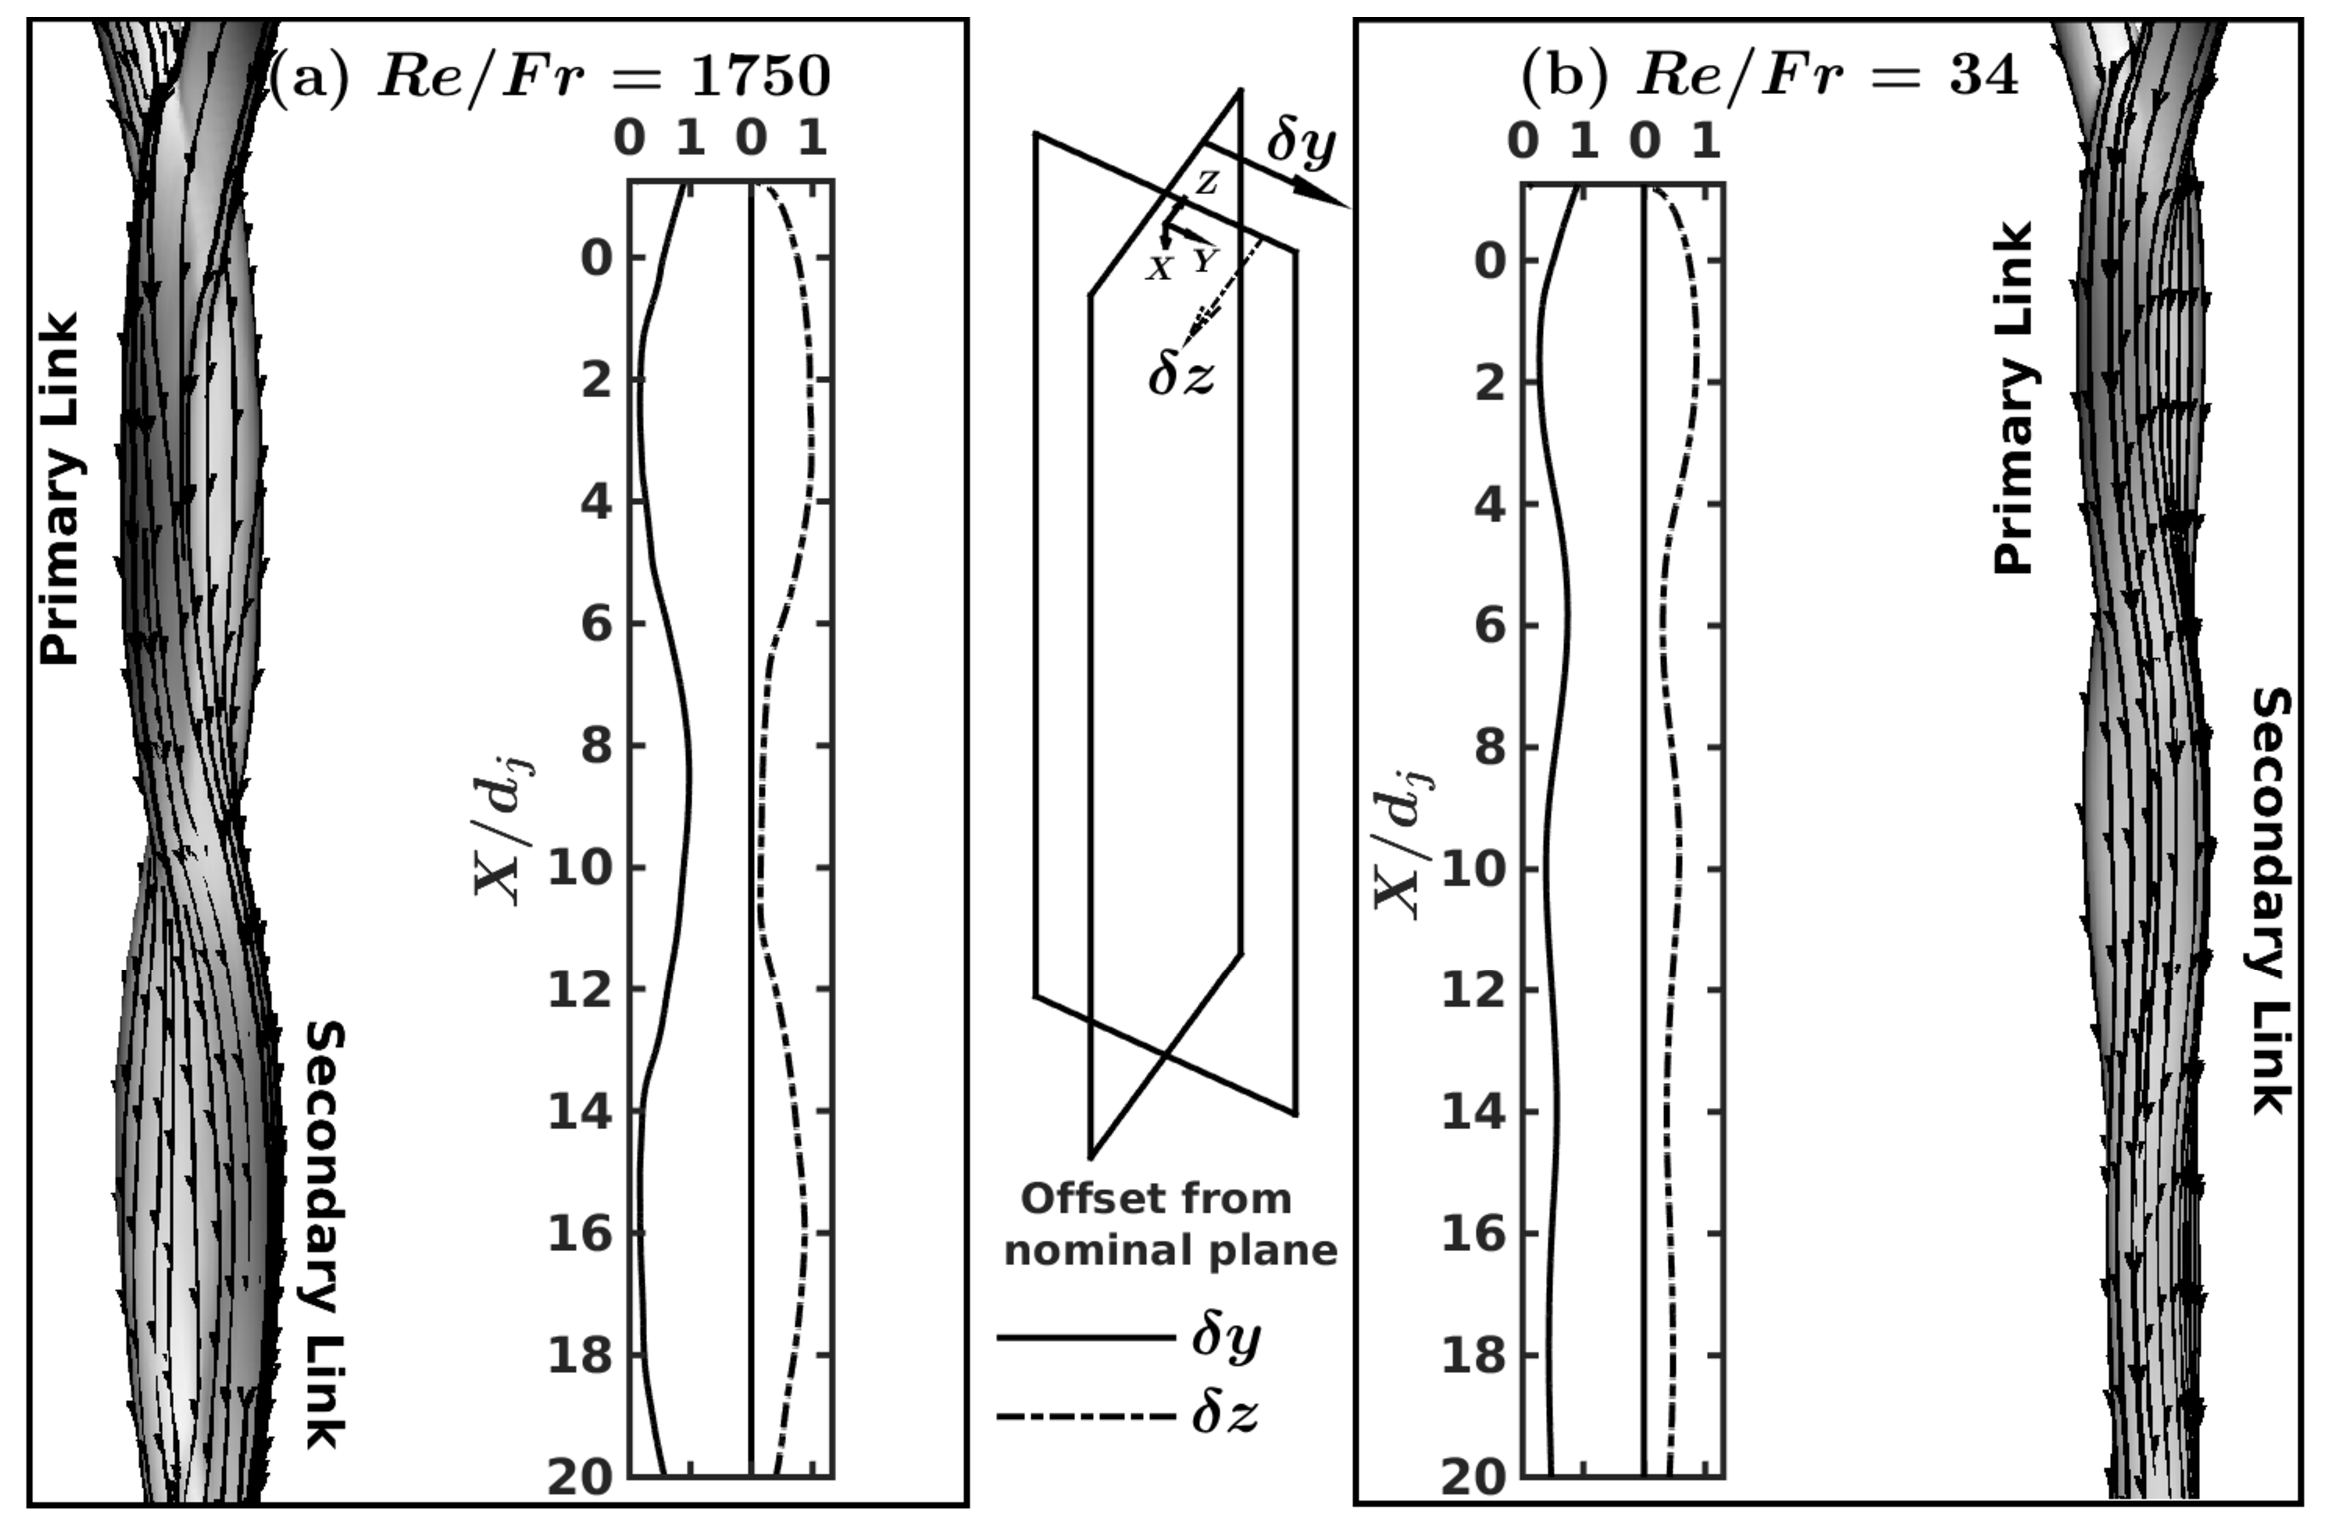
\includegraphics[width=\linewidth]{fig1}
	\caption{}
	\label{Figure::stream}
\end{figure}
\lipsum[1]
\subsection{Details of streamlines for the chain}
\lipsum[1]
\begin{figure}[H]
	\centering
	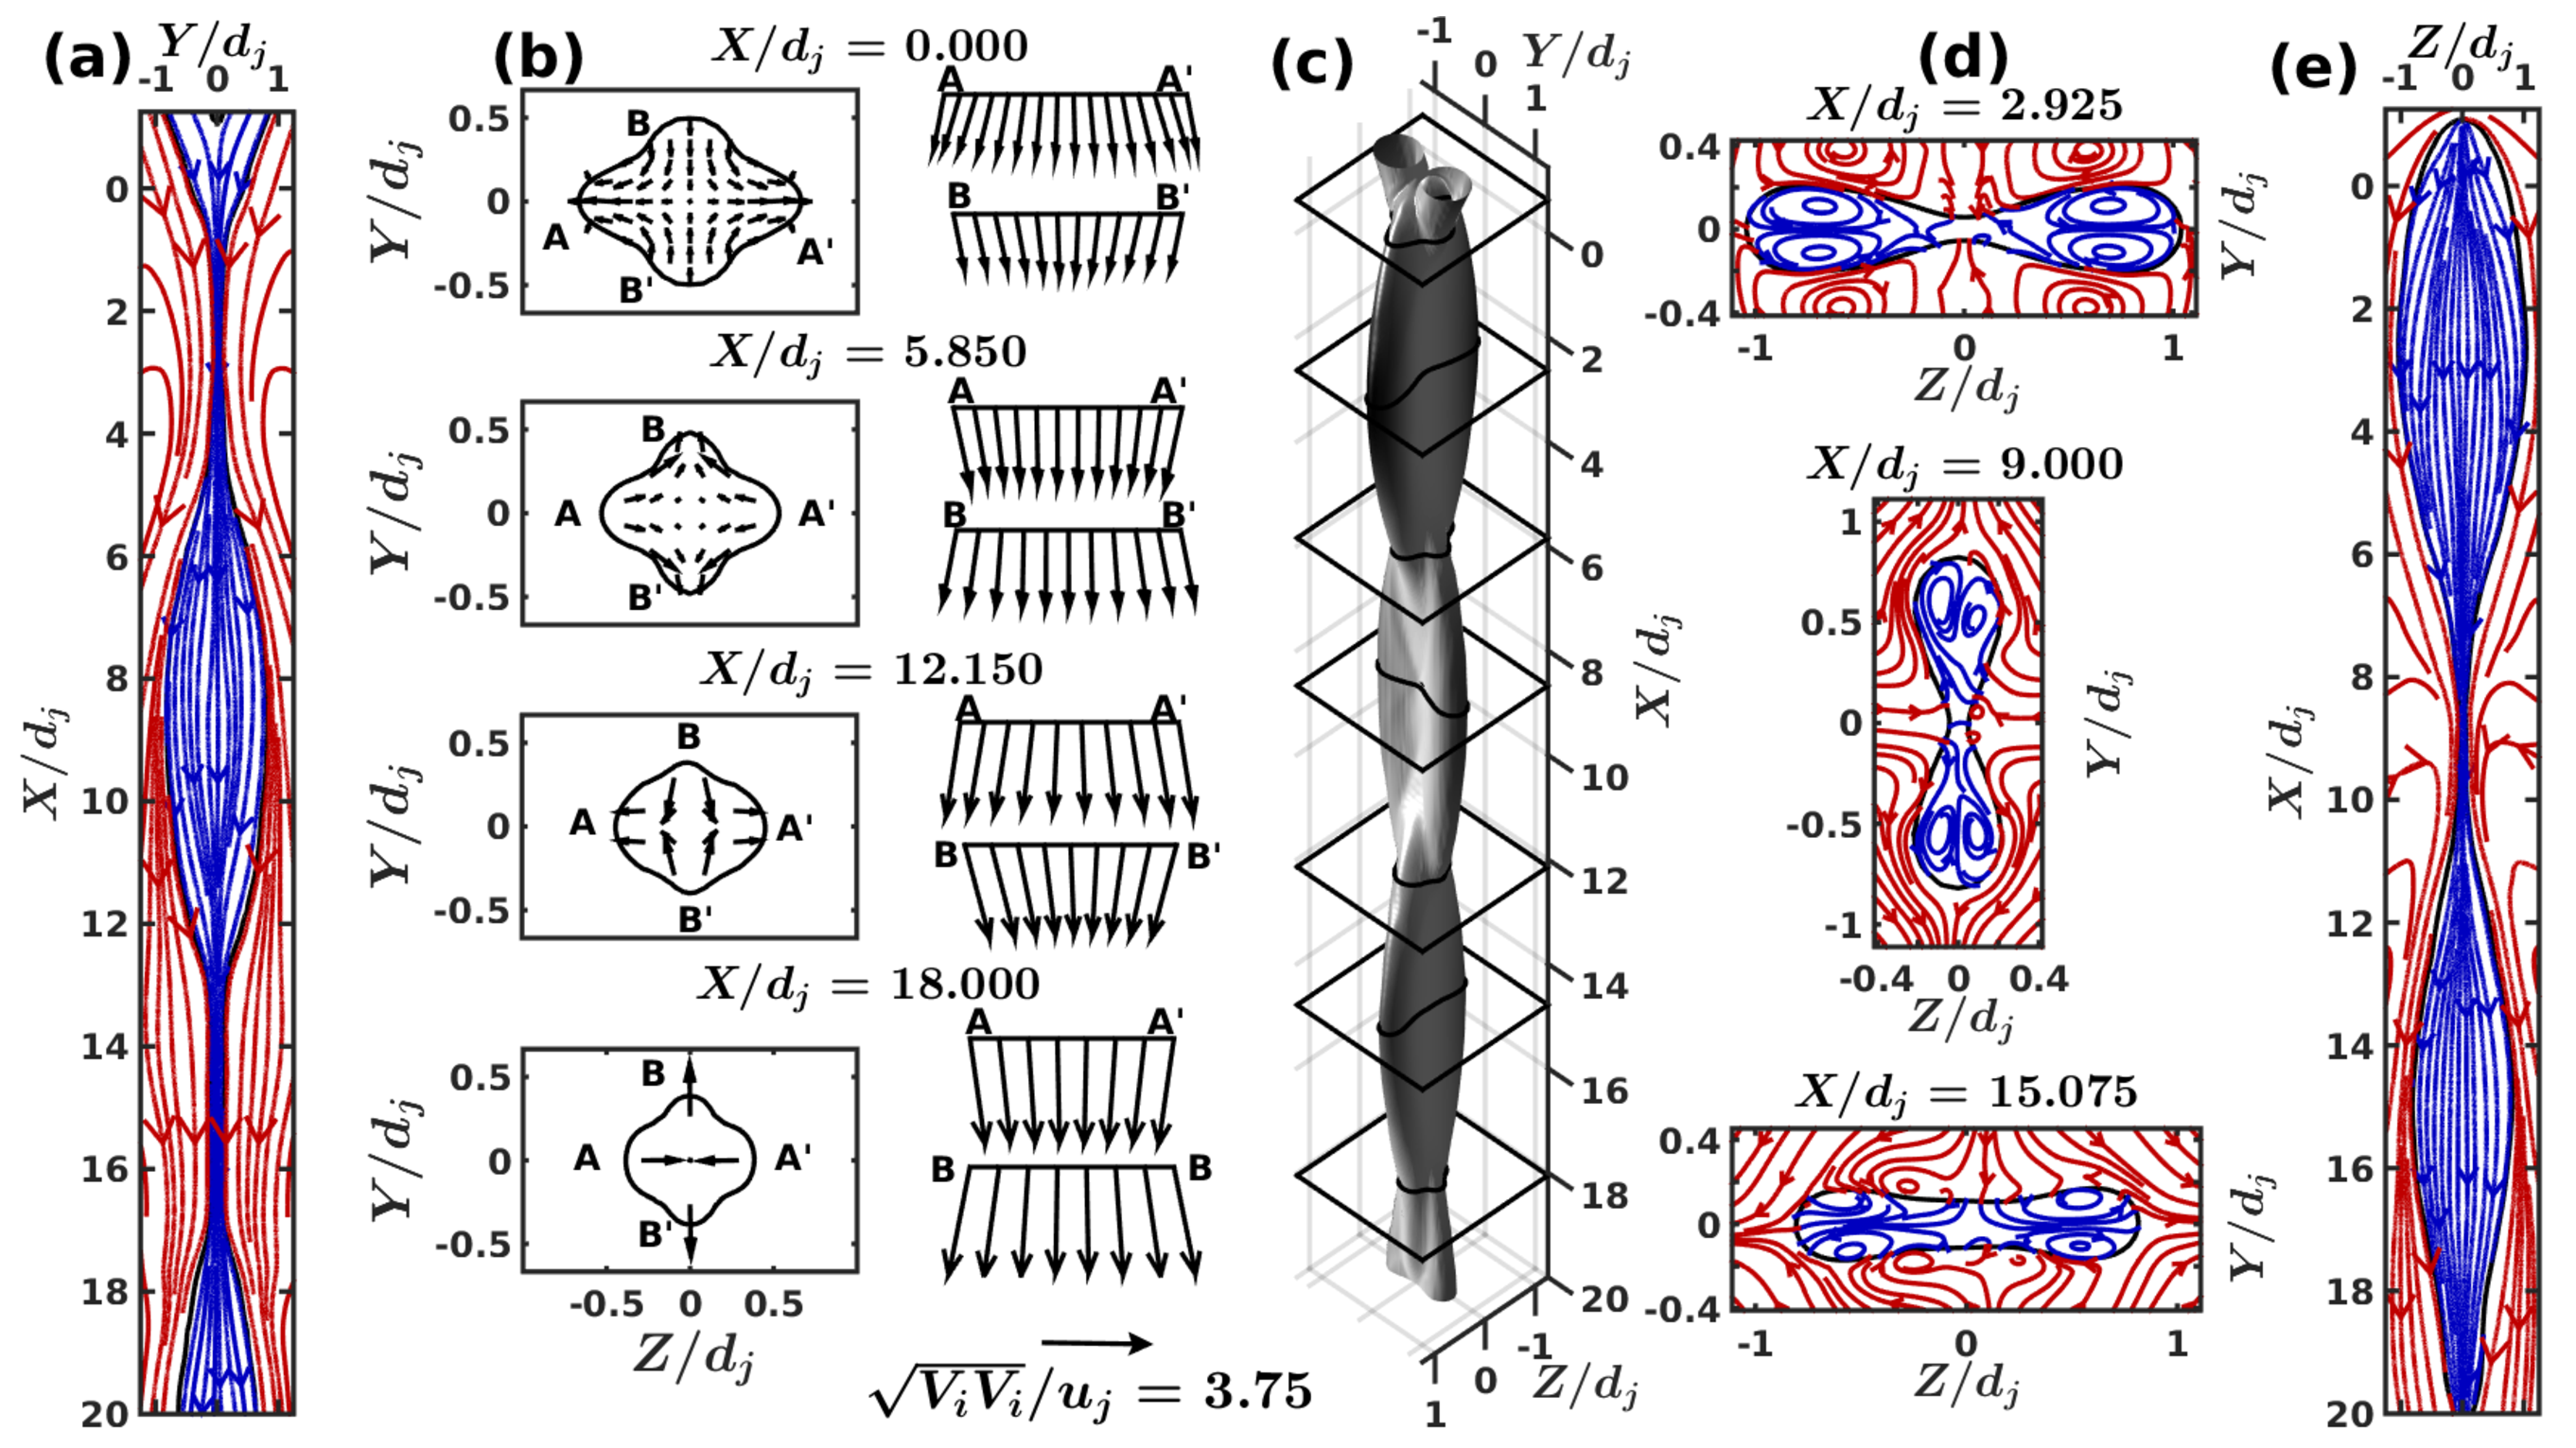
\includegraphics[width=\linewidth]{streamlinesDetails}
	\caption{}
	\label{Figure::streamDetails}
\end{figure}
\lipsum[1]
\nocite{*}
\bibliography{chains}

\end{document}